\documentclass[compress,9pt]{beamer}
%%%%%%% PACKAGES %%%%%%%%%
\usepackage[backend=biber,style=authoryear,bibstyle=authoryear,natbib=true,
giveninits=true,uniquename=false,uniquelist=false,maxcitenames=2,date=year,
maxbibnames=99,url=false]{biblatex}
\addbibresource{Thèse.bib}
\usepackage{tikz}
\usepackage[T1]{fontenc}
\usepackage[utf8]{inputenc}
\usepackage[french]{babel}
\usepackage{amsfonts}
\usepackage{amssymb}
\usepackage{lmodern}
\usepackage[absolute,overlay]{textpos}
\usepackage{contour}
\usepackage{ulem}
\usepackage{xcolor}
\usepackage{newunicodechar}
\usepackage{multirow}
\usepackage{setspace}
\usepackage{pifont}
\usepackage{appendixnumberbeamer}
\hypersetup{colorlinks=true,linkcolor=lightgray,filecolor=magenta,urlcolor=cyan,citecolor=cyan}
%%%%%%% PARAMETERS %%%%%%%%%
	%%%%%% CITE PARAMETERS %%%%%%%%%%%
		\AtEveryCitekey{\clearfield{title}\clearfield{note}\clearfield{pages}\clearlist{location}									    \clearlist{publisher}\clearname{editor}\clearfield{issn}\clearfield{doi}}
		\renewcommand*{\multicitedelim}{\\}
		\renewcommand{\footfullcite}[1]{\footnote[frame]{\fullcite{#1}}}
		\def\bibfont{\tiny}			% Réduit la taille de la police dans les références biblio
	%%%%%% THEME %%%%%%%%
		\usetheme{Madrid}
		\useoutertheme[subsection=false]{miniframes}
		\usefonttheme{structurebold}
		\usepackage{etoolbox}
		\makeatletter
		\patchcmd{\slideentry}{\advance\beamer@xpos by1\relax}{}{}{}
		\def\beamer@subsectionentry#1#2#3#4#5{\advance\beamer@xpos by1\relax}%
		\makeatother
		\definecolor{myblue}{RGB}{143, 174, 217}%{120,150,200}
		\usecolortheme[named=myblue]{structure}
		\beamertemplatenavigationsymbolsempty 
		\setbeamerfont{page number in head/foot}{size=\tiny}
		\setbeamerfont{section in head/foot}{size=\scriptsize}
		\setbeamerfont{section in toc}{size=\footnotesize}
		\setbeamerfont{subsection in toc}{size=\tiny}
		\setbeamerfont{frametitle}{size=\large}
		\setbeamerfont{block title}{size=\normalsize}
		\setbeamerfont{block body}{size=\normalsize}
		\setbeamertemplate{footline}[frame number]
		\setbeamertemplate{footcite}{site=\tiny}
		%transparence animations
		\setbeamercovered{transparent}
	%%%% ??
	\newcommand{\cmark}{\ding{51}}
	\newcommand{\xmark}{\ding{55}}
	\newcommand\Wider[2][3em]{%
	\makebox[\linewidth][c]{%
	  \begin{minipage}{\dimexpr\textwidth+#1\relax}
	  \raggedright#2
	  \end{minipage}%
	  }%
	}
%%%%%%%% TITLE %%%%%%%%%
\title{Comment valoriser les données anciennes pour l’analyse fréquentielle des crues : application au Rhône à Beaucaire de 1500 à 2020}
\author{Mathieu LUCAS}
\date{3 juillet 2023}
%%%%%%%%% MAIN PART %%%%%%%%%%
\begin{document}

%%%%%%%% PDG %%%%%%%%%
%{
\usebackgroundtemplate{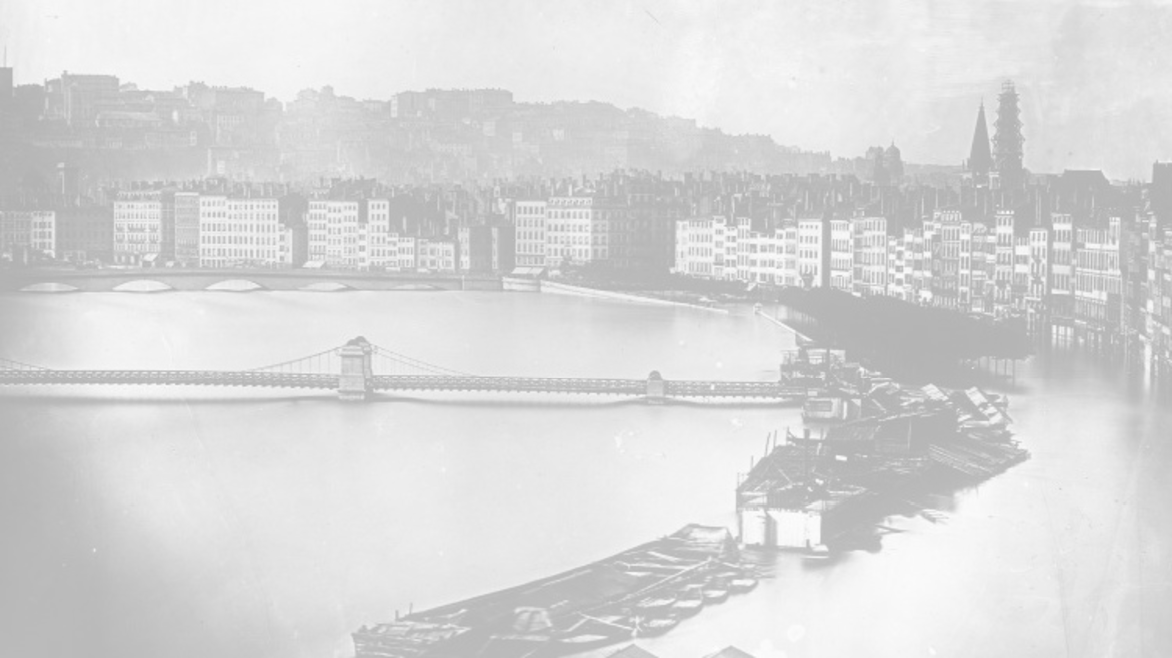
\includegraphics[height=\paperheight,width=\paperwidth]{./Figures/Back.pdf}}

\begin{frame}[plain]
     \vspace{10pt}
%     \vfill
     
\includegraphics[height= .5cm]{./Figures/CNR.png}	\hspace{4pt}
     
\includegraphics[height= .6cm]{./Figures/h2o.png}  \hspace{4pt}
     
\includegraphics[height= .5cm]{./Figures/INRAE.jpg}  \hspace{4pt}
     
\includegraphics[height= .6cm]{./Figures/lyon1.png}  \hspace{4pt}
     
\includegraphics[height= .6cm]{./Figures/MEGA.png}  \hspace{4pt} 
     
\includegraphics[height= .6cm]{./Figures/OSR.jpg}  \hspace{4pt}
     
\includegraphics[height= .6cm]{./Figures/Eu.jpg}  
     \centering
%     \begin{beamercolorbox}[sep=10pt,center,colsep=-4bp,rounded=true,shadow=true]{institute}
%     \end{beamercolorbox}
	\vspace{20pt}
     {\usebeamercolor[fg]{titlegraphic}\inserttitlegraphic\par}
     \begin{beamercolorbox}[sep=10pt,center,colsep=-4bp,rounded=true,shadow=true]{title}
        \usebeamerfont{title}\inserttitle\par%
%        \ifx\insertsubtitle\@empty%
%        \else%
%        \vskip0.25em%
%        {\usebeamerfont{subtitle}\usebeamercolor[fg]{subtitle}\insertsubtitle\par}%
%      \fi%     
     \end{beamercolorbox}%
     \vskip1em\par
     \begin{beamercolorbox}[sep=10pt,center,colsep=-4bp,rounded=true,shadow=true]{author}
%        \usebeamerfont{author}
        \Large{\insertauthor}
     \end{beamercolorbox}
%    \begin{beamercolorbox}[sep=5pt,center,colsep=-4bp,rounded=true,shadow=true]{author}
%    \centerize
    3 juillet 2023
   
  \flushleft \noindent \footnotesize Devant le jury composé de :\\
%\vspace{\stretch{1}}
%\begin{adjustwidth}{-0.8cm}{}
	\begin{center}
	\noindent \footnotesize{
	\begin{tabular}{llrl}
	    	\textsc{Carreau} & Julie & Professeure adjointe, Université de Montréal & Rapporteure\\
	    	\textsc{Llasat} & Maria-Carmen & Professeure, Université de Barcelone & Rapporteure\\
	    	\textsc{Favre}	& Anne-Catherine & Professeure, Université Grenoble Alpes & Examinatrice\\
	      	\textsc{Payrastre} & Olivier & IDTPE, Université Gustave Eiffel & Examinateur\\
	      	\textsc{Riviere} & Nicolas & Professeur, INSA Lyon & Examinateur\\
	      	\textsc{Ribereau} & Pierre & Maître de Conférences,  Université Lyon 1 & Examinateur\\
	      	\textsc{Lang} & Michel & ITPEHC , INRAE Villeurbanne & Directeur de thèse \\
	      	\textsc{Le Coz} & Jérôme & ICPEF, INRAE Villeurbanne & Co-encadrant\\
	      	\textsc{Renard} & Benjamin& Chargé de Recherche, INRAE Aix-en-Provence& Co-encadrant\\
	      	\textsc{Pierrefeu} & Gilles & Ingénieur, CNR & Invité \\
	\end{tabular}
	}
	\end{center}

%    \end{beamercolorbox}
%     \begin{beamercolorbox}[sep=8pt,center,colsep=-4bp,rounded=true,shadow=true]{date}
%        \usebeamerfont{date}\insertdate
%     \end{beamercolorbox}\vskip0.5em


\end{frame} 
}
\setcounter{page}{1}
\section{Introduction}
	\subsection{Le risque de crue}
	
	%%%%%%%%% 1 %%%%%%%%%
	\begin{frame}[c]
		\frametitle{Le risque de crue}
      	\begin{minipage}{0.4\textwidth}
      		\begin{itemize}
      			\item<1->[$\vartriangleright$] Type de catastrophe naturelle le plus fréquent dans le monde au XXI\textsuperscript{ème} siècle\footfullcite{undrr_human_2020}
      			\vspace{10pt}
      			\item<2->[$\vartriangleright$] Plus de 104 000 morts de 2000 à 2019
      		\end{itemize}
      	\end{minipage}
      	\begin{minipage}{0.59\textwidth}
      		\begin{center}
      			\item \includegraphics<1>[width= .8\textwidth]{./Figures/1-Crue2005TyrolBBA-Imst.jpg}  
				\item \includegraphics<2>[width= .8\textwidth]{./Figures/2-UNDRR.png}  
      		\end{center}
      	\end{minipage}
	\end{frame}
		
	\subsection{L'estimation du risque}
	
	%%%%%%%%% 2 %%%%%%%%%
	\begin{frame}%[c]
		\frametitle{L'estimation du risque}
		Nécessité de caractériser statistiquement l'aléa de crue :\\
    		\vspace{10pt}
      	\begin{minipage}{0.45\textwidth}  		
      		\begin{itemize}
      			\item<2->[$\vartriangleright$] Plan de prévention du risque inondation
      			 $\Rightarrow$ \og\textit{événement le plus important connu ou} [...] \textit{évènement théorique de \textbf{fréquence centennale}, si ce dernier est plus important}\fg{} \footfullcite{Code de l'environnement (France); article R562-11-3}
      			\vspace{10pt}
      			\item<4>[$\vartriangleright$] Dimensionnement d'infrastructures à risque
      			$\Rightarrow$ \textbf{périodes de retour jusqu'à 10~000 ans}
      		\end{itemize}
      	\end{minipage}
      	\begin{minipage}{0.5\textwidth}
      		\begin{center}
      		    \includegraphics<2>[width = .9\textwidth]{./Figures/3-PPRI_lyon0.pdf}
				\includegraphics<3>[width = .9\textwidth]{./Figures/4-PPRI_lyon.pdf}  
				\includegraphics<4>[width = .8\textwidth]{./Figures/5-Grangent.jpg} 
      		\end{center}
      	\end{minipage}
	\end{frame}
	
	%%%%%%%%% 3 %%%%%%%%%    %crues = réalisations + concept de période de retour
	\begin{frame}%[c]
		\frametitle{L'estimation du risque}
		Il est possible de modéliser les processus de crues à l'aide de distributions statistiques\\
      	\vspace{15pt}			
		\begin{center}
			\includegraphics[width = .8\textwidth]{./Figures/6-Réalisations.pdf} 
		\end{center}
		\vspace{10pt}
		\begin{itemize}
			\item<2->[$\vartriangleright$] Les observations de crues $(x_1,...,x_n)$ sont des réalisations d'une variable aléatoire $X$ 
		\end{itemize}
	\end{frame}
	
	\subsection{Analyse fréquentielle}
	%%%%%%%%% 4 %%%%%%%%%    Théorie des valeurs extrêmes
	\begin{frame}%[c]
		\frametitle{Théorie des valeurs extrêmes}
		\vfill
		\textbf{La théorie des valeurs extrêmes} nous donne le cadre pour modéliser ces processus \footfullcite{fisher_limiting_1928}\textsuperscript{;}\footfullcite{gumbel_statistics_1958}
		\vfill
		\begin{itemize}
			\item<2-> [$\vartriangleright$] On a $X_1,...,X_n$ une séquence de \textbf{variables aléatoires} $iid$\\
			\textit{Par exemple une série temporelle de débits}
			\vspace{5pt}
			\item<3-> [$\vartriangleright$] La valeur maximale sur un bloc de $n$ valeurs est $M_n = max(X_1,...,X_n)$\\Par exemple une série de maximum annuels de débit
			\vspace{5pt}
			\item<4> [$\vartriangleright$] La distribution de $M_n$ quand $n\rightarrow \infty$ converge vers la loi généralisée des valeurs extrêmes : $GEV(\mu,\sigma,\xi)$

		\end{itemize}	
	\end{frame}
	
	%%%%%%%%% 5 %%%%%%%%%
	\begin{frame}%[c]
		\frametitle{Analyse fréquentielle des crues}
		\begin{center}
			\includegraphics<1>[width = .8\textwidth]{./Figures/Qamax.pdf} 
			\includegraphics<2>[width = .8\textwidth]{./Figures/Qamax_GEV.pdf} 
			\includegraphics<3>[width = .8\textwidth]{./Figures/Qamax_GEV_Q100.pdf} 
		\end{center}
	\end{frame}
	
	%%%%%%%%% 6 %%%%%%%%%
	\begin{frame}%[c]
		\frametitle{Prédétermination des crues}
		\vfill
		Domaine de la \textbf{prédétermination} $\neq$ \textbf{prévision}\\
		\vspace{10pt}
		\onslide<1-> Le débit d'une crue de \textbf{période de retour} $T$
		\vspace{10pt}
      	\begin{itemize}
			\item<2->[$\vartriangleright$] a une probabilité $p = 1/T$ d'être dépassé chaque année
			\vspace{2pt}
			\item<3->[$\vartriangleright$] a une probabilité $p' = 1 - 1/T$ de ne pas être dépassé
		\end{itemize}
		\vfill
		\centering
		\includegraphics<4->[width = .3\textwidth]{./Figures/Attention.png} 
		\vfill
		\begin{itemize}
			\item<5->[$\vartriangleright$] Une crue centennale n'apparait pas tous les 100 ans
			\item<5->[$\vartriangleright$] On peut observer 2 crues centennales deux années de suite
		\end{itemize}
	\end{frame}
	
	%%%%%%%%% 7 %%%%%%%%%
	\begin{frame}%[c]
		\frametitle{Analyse fréquentielle et incertitudes}
		Ces estimations affectées par des incertitudes :
		\vfill
      	\begin{itemize}
      		\item<2-7>[$\vartriangleright$] \textbf{Hypothèses de modélisation} : \onslide<3-7>{choix d'une distribution, stationnarité...}
      		\vspace{5pt}
      		\item<4-7>[$\vartriangleright$] \textbf{Données d'entrée} : \onslide<5-7>{estimation du débit des cours d'eau}
      		\vspace{5pt}
      		\item<6-7>[$\vartriangleright$] \textbf{Échantillonnage} : \onslide<7>{longueur limitée des échantillons de crues}
      	\end{itemize}
      	\vfill
      	\centering
      	\onslide<8> Leur détermination est \textbf{essentielle} pour
      	\begin{itemize}
      		\item<9>[$\vartriangleright$] la prise de décision (infrastructures à risque, arrêtés Cat. nat...)
      		\vspace{5pt}
      		\item<10>[$\vartriangleright$] comprendre l'apport des informations historiques
      	\end{itemize}
      	 notamment pour la prise de décision
	\end{frame}
	
	\subsection{Incertitude hydrométrique}
	%%%%%%%%% 8 %%%%%%%%%
	\begin{frame}[c]
		\frametitle{Incertitudes hydrométriques}
      	Le débit des cours d'eau ne peut être mesuré en continu
      	\begin{itemize}
      		\item<2->[$\vartriangleright$] Mesure de la hauteur d'eau
		\end{itemize}
		\vspace{3pt}
		\begin{center}
			\includegraphics<3>[width = .3\textwidth]{./Figures/LogoHydro.pdf}
			\includegraphics<3>[width = .6\textwidth]{./Figures/LimniVienne.png}
			\includegraphics<4>[width = .7\textwidth]{./Figures/Hydrom1.pdf}
			\includegraphics<5>[width = .7\textwidth]{./Figures/Hydrom2.pdf}
			\includegraphics<6>[width = .7\textwidth]{./Figures/4Jau.pdf}
			\includegraphics<7>[width = .7\textwidth]{./Figures/Hydrom3.pdf}
			\includegraphics<8>[width = .7\textwidth]{./Figures/Hydrom4.pdf}
		\end{center}

	\end{frame}
	
	%%%%%%%%% 9 %%%%%%%%%
	\begin{frame}%[c]
		\frametitle{Incertitudes hydrométriques}
		\begin{center}\begin{itemize}
			\item<1->[\Huge{$\textcolor{green}{\checkmark}$}] Méthodes de calcul des incertitudes à chaque étape\\
			\vspace{10pt}
			\item<2>[\Huge{$\textcolor{red}{X}$}] Propagation complète et homogène des incertitudes
		\end{itemize}\end{center}	
		\vspace{10pt}
		\begin{center}
			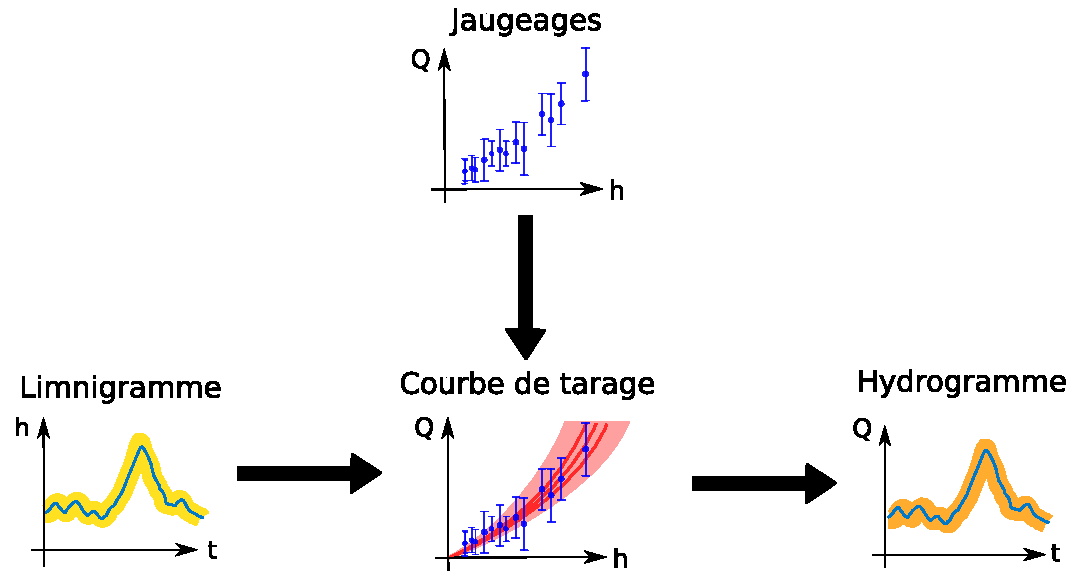
\includegraphics[width = .7\textwidth]{./Figures/Hydrom4.pdf}
		\end{center}
	\end{frame}
	
	\subsubsection{CT}
	%%%%%%%%% 11 %%%%%%%%%	
	\begin{frame}
    	\frametitle{Estimation des courbes de tarage}
    		Équation générale de la courbe de tarage : 
    		\begin{equation}
    			Q = \textcolor{red}{a}(h-b)^{\textcolor{red}c}
    		\end{equation}
		\vspace{1cm}
		\begin{minipage}{.4\textwidth}
			\begin{itemize}
				\item<2->[$\vartriangleright$] Détermination des contrôles hydrauliques
				\vspace{0.5cm}
				\item<3->[$\vartriangleright$] Formules hydrauliques selon le type de contrôle (Manning-Strickler, loi de seuil...)
			\end{itemize}
		\end{minipage}
		\begin{minipage}{.55\textwidth}
			\begin{center}
				\includegraphics<2>[width = \textwidth]{./Figures/Controles.jpg} 
				\vspace{5pt}
				\onslide<3-> $Q = \underbrace{Ks\sqrt{S}Bc}_{\mathrm{\textcolor{red}{a}}}(h-b)\underbrace{^{5/3}}_{\mathrm{\textcolor{red}{c}}}$
			\end{center}
		\end{minipage}
    \end{frame}
    
    %%%%%%%%% 12 %%%%%%%%%	
	\begin{frame}
    	\frametitle{Estimation des courbes de tarage}
		Estimation bayésienne des paramètres de la courbe de tarage : \textbf{BaRatin}\footfullcite{le_coz_combining_2014}\\
		\vfill		
		\begin{center}
			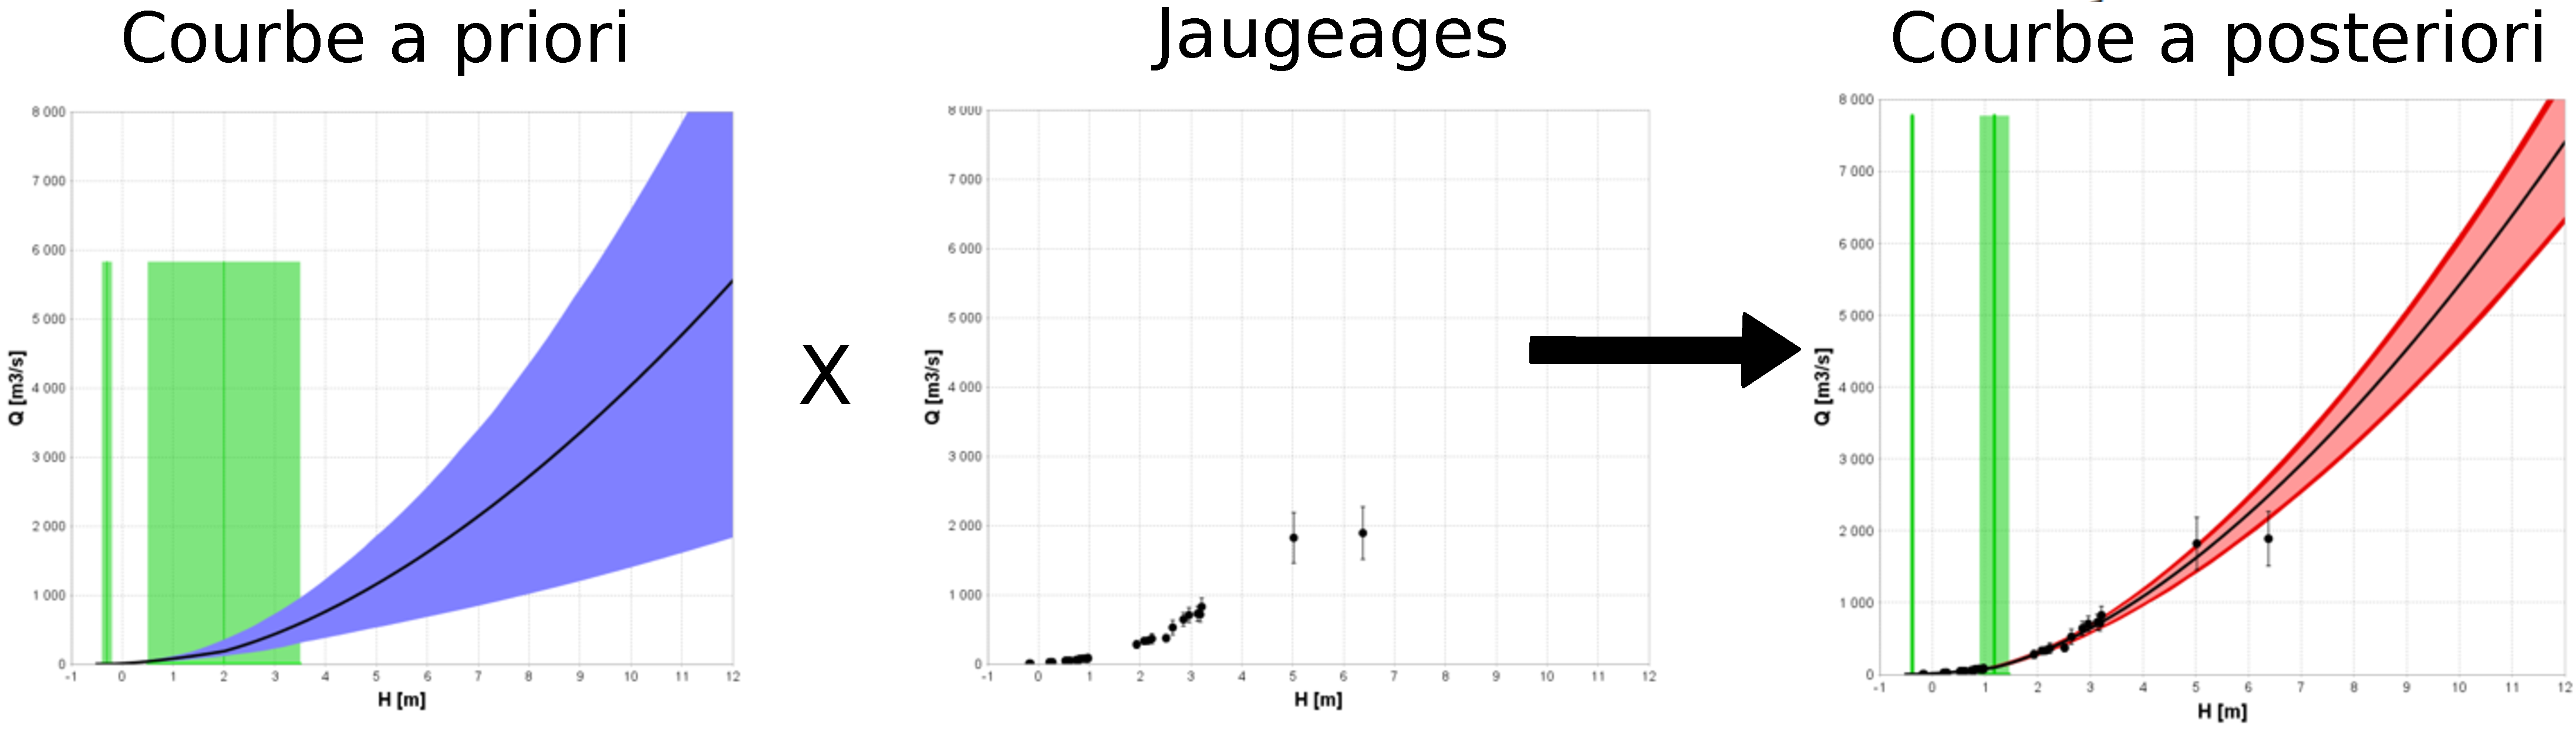
\includegraphics[width = .8\textwidth]{./Figures/Baratin.pdf} 
		\end{center}
%		\begin{minipage}{.4\textwidth}
			\begin{itemize}
				\item<1->[$\vartriangleright$] Courbe \textbf{\textit{a priori}} $\rightarrow$ connaissance hydraulique de la station\\		
				\vspace{0.5cm}
				\item<2->[$\vartriangleright$] Courbe \textbf{\textit{a posteriori}} $\rightarrow$ combinaison de la courbe \textbf{\textit{a priori}} et des jaugeages \\		
				\vspace{0.5cm}
				\item<3->[$\vartriangleright$] Prise en compte de l'incertitude des jaugeages
			\end{itemize}
%		\end{minipage}
%		\begin{minipage}{.55\textwidth}
%			\begin{center}
%				\includegraphics<2>[width = \textwidth]{./Figures/Baratin.pdf} 
%			\end{center}
%		\end{minipage}
	\end{frame}

	\subsubsection{Détarages}
	%%%%%%%%% 12 %%%%%%%%%
	\begin{frame}%[c]
		\frametitle{Détarages}
		Ruptures dans la relation hauteur/débit\\
		\vspace{15pt}
		\begin{center}
			\includegraphics<1>[width = .45\textwidth]{./Figures/Detar1.pdf} 
			\includegraphics<2>[width = .45\textwidth]{./Figures/Detar2.pdf} 
			\includegraphics<3>[width = .45\textwidth]{./Figures/Detar3.pdf} 
		\end{center}
	\end{frame}
	
	%%%%%%%%% 11 %%%%%%%%%
	\begin{frame}%[c]
		\frametitle{Segmentation des jaugeages}
		Méthode bayésienne de détection des détarages \footfullcite{darienzo_detection_2021}\\
		\vspace{10pt}
		\begin{center}
			\includegraphics<1>[width = .3\textwidth]{./Figures/CT1.pdf} 
			\includegraphics<2>[width = .3\textwidth]{./Figures/CT2.pdf} 
			\includegraphics<3>[width = .4\textwidth]{./Figures/CT3.pdf} 
			\includegraphics<4>[width = .4\textwidth]{./Figures/CT4.pdf} 
			\includegraphics<5->[width = .7\textwidth]{./Figures/Matt.pdf}
			\vspace{10pt}
			\begin{itemize}
				\item<6->[$\vartriangleright$]Prise en compte des incertitudes des jaugeages et des courbes de tarage\\
				\item<7->[$\vartriangleright$] Incertitude sur les dates de détarage $\rightarrow$ choix utilisateur
			\end{itemize}
		\end{center}
	\end{frame}
	
	\subsubsection{CT multi}	
	%%%%%%%%% X %%%%%%%%%
    \begin{frame}
    Modèle de courbes de tarage multipériodes : \textbf{BaRatin SPD} (Stage-Period-Discharge)\footfullcite{mansanarez_shift_2019}
    \vfill
    	\frametitle{Estimation des courbes de tarage}
		\begin{minipage}{.44\textwidth}
		\begin{itemize}
			\item<1->[$\vartriangleright$] Périodes avec peu/pas de jaugeages
			\vspace{0.5cm}
			\item<2->[$\vartriangleright$] Paramètres constants entre périodes ? $\Rightarrow$ expertise terrain
			\vspace{0.5cm}
			\item<3->[$\vartriangleright$] Transfert d'informations entre périodes
			\vspace{0.5cm}
			\item<4->[$\vartriangleright$] Pas de "recyclage"
			\end{itemize}
		\end{minipage}
		\begin{minipage}{.55\textwidth}
			\begin{center}
				\includegraphics<3->[width = \textwidth]{./Figures/Spd.jpg} 	
			\end{center}
		\end{minipage}    	   	
    \end{frame}
    
    	%%%%%%%%% X %%%%%%%%%
	\begin{frame}%[c]
		\frametitle{Incertitudes hydrométriques}
		\begin{center}
			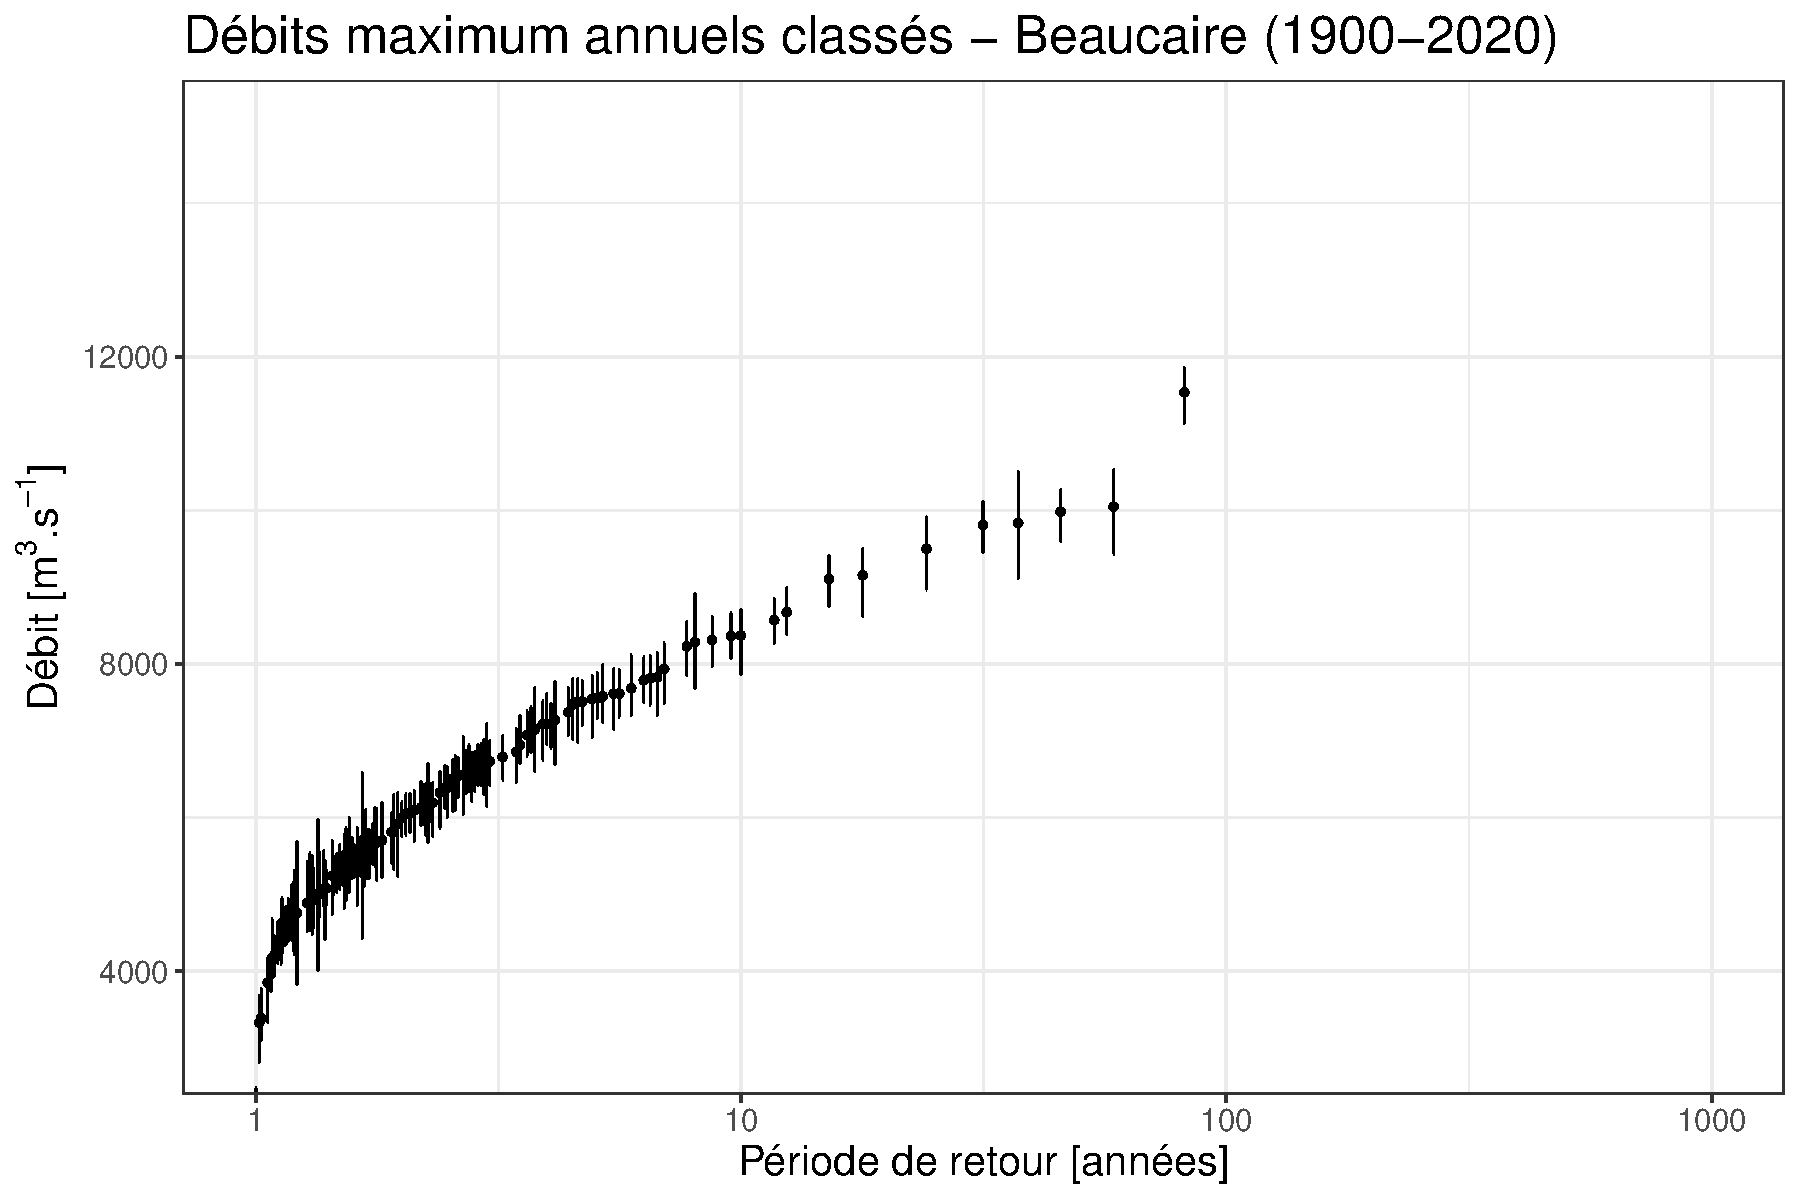
\includegraphics[width = .8\textwidth]{./Figures/Qamax_uQ.pdf} 
		\end{center}
	\end{frame}
	
	\subsection{Incertitude d'échantillonnage}    
    %%%%%%%%% 12 %%%%%%%%%
	\begin{frame}%[c]
		\frametitle{Incertitude d'échantillonnage}
      	\begin{itemize}
			\item<2->[$\vartriangleright$] Longueur des chroniques limitée $\Rightarrow$ 60 ans en moyenne en France\footfullcite{le_coz_quantifying_2017}
			\vspace{2pt}
			\item<3->[$\vartriangleright$] Périodes de retour ciblées plus grandes : 100, 1000, 10 000 ans
		\end{itemize}
      	\begin{center}
      		\includegraphics<1>[width = .3\textwidth]{./Figures/LogoHydro.pdf}
      		\includegraphics<2-3>[width = .6\textwidth]{./Figures/NbStationsHydro.pdf}
			\includegraphics<4>[width = .6\textwidth]{./Figures/Qsample1.pdf}
			\includegraphics<5->[width = .6\textwidth]{./Figures/Qsample2.pdf}\phantom{s}\\
			\vfill
			\centering
			\centering
			\onslide<6-> Il est possible\footfullcite{coles_classical_2001}	et nécessaire d'\textbf{estimer cette incertitude} 	
		\end{center}
	\end{frame}
	
	%%%%%%%%% X %%%%%%%%%
	\begin{frame}[c]
		\frametitle{Incertitude d'échantillonnage}
		\vspace{5pt}
		Élargir le jeu de données $\Rightarrow$ Diminuer l'incertitude d'échantillonnage\\
		\vspace{10pt}
		\begin{minipage}[t]{0.49\textwidth}
			\begin{itemize}
				\centering
				\item<2->[$\vartriangleright$] \textbf{Spatialement}
			\end{itemize}
			\vspace{2pt}
			\centering
			\includegraphics<2->[width = .6\textwidth]{./Figures/Regional.pdf}\phantom{s}\\
			\vspace{2pt}
			\onslide<2->\scriptsize{Bassins versants méditerranéens\footfullcite{gaume_bayesian_2010}} \\
			\vspace{2pt}
			\onslide<3-> \normalsize{Homogénéité régionale}
		\end{minipage}
		\begin{minipage}[t]{0.49\textwidth}
			\begin{itemize}
				\centering
				\item<4->[$\vartriangleright$] \textbf{Temporellement}
			\end{itemize}
			\vspace{7pt}
			\centering
			\includegraphics<4>[width = \textwidth]{./Figures/HistoFloods0.pdf}%\phantom{s}\\
			\includegraphics<5-6>[width = \textwidth]{./Figures/HistoFloods.pdf}%\phantom{s}\\
			\includegraphics<7->[width = .95\textwidth]{./Figures/HistoFloods1.pdf}\phantom{s}\\
			\vspace{1pt}
			\onslide<4-> \scriptsize{Red River of the North à Winnipeg, Canada \footfullcite{st_george_paleofloods_2020}} \\
			\vspace{2pt}
			\onslide<6-> \normalsize{Homogénéité temporelle}
		\end{minipage}
	\end{frame}
	
	%%%%%%%%% X %%%%%%%%%
	\begin{frame}%[c]
		\frametitle{Crues historiques et analyse fréquentielle}
		\centering
		Les données de crues historiques peuvent prendre des formes diverses :
		\vfill
		\begin{minipage}{0.49\textwidth}
	      	\begin{itemize}
	      		\item<2->[$\vartriangleright$] Relevés hydrométriques non-bancarisés
	      		\item<3->[$\vartriangleright$] Repères de crue
	      		\item<4->[$\vartriangleright$] Témoignages 
	      		\item<5->[$\vartriangleright$] Reconstructions issues de divers proxys
	      	\end{itemize}
      	\end{minipage}
      	\begin{minipage}{.45\textwidth}
      		\begin{center}
      		\includegraphics<3>[width = .5\textwidth]{./Figures/RepAvi.jpg} 
      		\includegraphics<4>[width = .8\textwidth]{./Figures/Parchemin.jpg} 
      		\includegraphics<5>[width = .4\textwidth]{./Figures/Sedim.pdf} 
      		\includegraphics<6>[width = .9\textwidth]{./Figures/Dendro.jpg} \phantom{s}\\
			\end{center}
      	\end{minipage}
      	\vfill
      	\centering
      	\onslide<6-> Données généralement sporadiques $\Rightarrow$ nécessitent des traitements statistiques adaptés
%      	\onslide<7-> Prise en compte complète et homogène des incertitudes \textbf{généralement oubliée}
	\end{frame}
	
	\subsection{Problématiques et objectifs}
	%%%%%%%%% X %%%%%%%%%	
	\begin{frame}
	    \frametitle{Problématiques}
		\begin{itemize}
		
			\item Comment estimer et propager l'ensemble des incertitudes hydrométriques ? 
			
			\item Quelle est la part de l'incertitude hydrométrique et de l'incertitude d'échantillonnage dans les quantiles de crue ?
			
			\item Quel est l'apport des divers types l'information historique ?
			
			\item Jusqu'à quel point l'ajout d'information historique permet-il de réduire l'incertitude des quantiles de crue ?
		\end{itemize}
	\end{frame}
	
	%%%%%%%%% X %%%%%%%%%	
	\begin{frame}
	    \frametitle{Objectifs}
	    \begin{itemize}
	    
	    \item Estimer et propager de façon complète et homogène les différentes sources d'incertitudes hydrométriques jusqu'aux séries de débit
	    
	    \item Estimer la part des différentes incertitudes lors de l'analyse fréquentielle
	    
	    \item  Mettre un point un modèle qui considère une incertitude sur le seuil de perception et la durée des échantillons de crues historiques
	    
	    \item Chiffrer l'apport de l'information historique lors de l'analyse fréquentielle
	    
	    \end{itemize}
	\end{frame}
	
	
\section{Cas d'étude}
	\subsection{Le Rhône à Beaucaire}
	{
    \setbeamercolor{background canvas}{bg=myblue}
    \begin{frame}
        \begin{center}
				\textcolor{white}{\Large \textbf{Le Rhône à Beaucaire}}\\
		 		\vspace{0.3cm}
		 		\textcolor{white}{\large \textbf{Collecte et caractérisation des données de crue}}\\
		 		\vspace{0.8cm}
		 		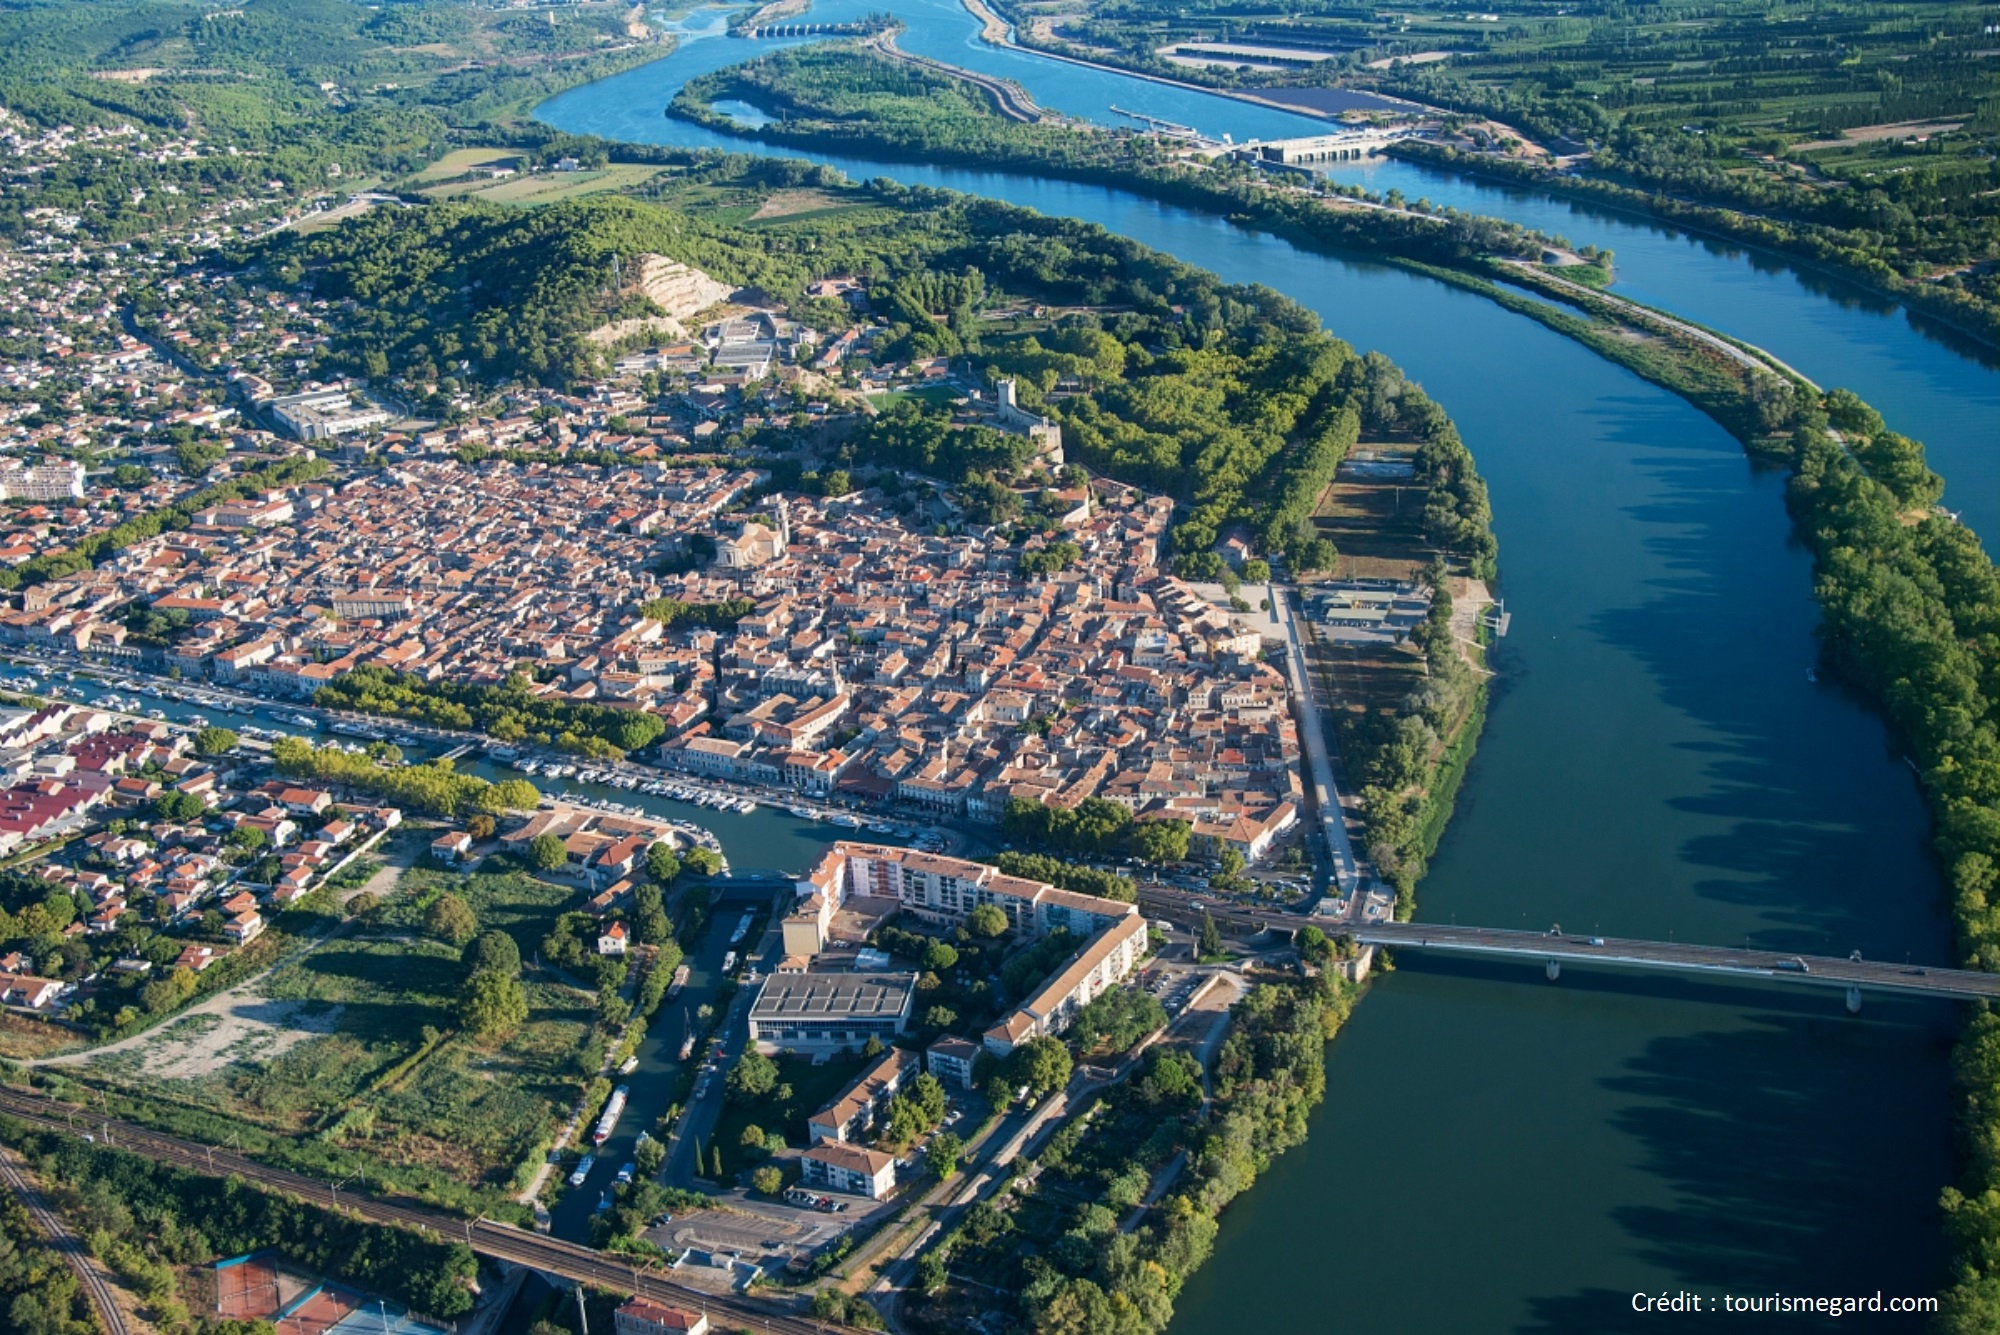
\includegraphics[width = .7\textwidth]{./Figures/BcrAerien.jpg} 
        \end{center}
    \end{frame}
    }
    	
    	\subsection{Station hydrométrique}
	%%%%%%%%% 19 %%%%%%%%%
	\begin{frame}%[c]
		\frametitle{Présentation de la station}
		\begin{minipage}{.55\textwidth}
			\begin{itemize}
				\item<1->[$\vartriangleright$] Bassin versant de 95 590 km²
				\vspace{5pt}
				\item<2->[$\vartriangleright$] Plus fort débit français
				\vspace{5pt}
				\item<3->[$\vartriangleright$] Apports variés et complexes : \og\textit{il comporte une infinité de nuances et de contrastes}\fg{}   \footfullcite{parde_regime_1925}
				\vspace{5pt}
				\item<4->[$\vartriangleright$] Dernière station du Rhône complet
			\end{itemize}
		\end{minipage}
		\begin{minipage}{.4\textwidth}
			\centering
	      	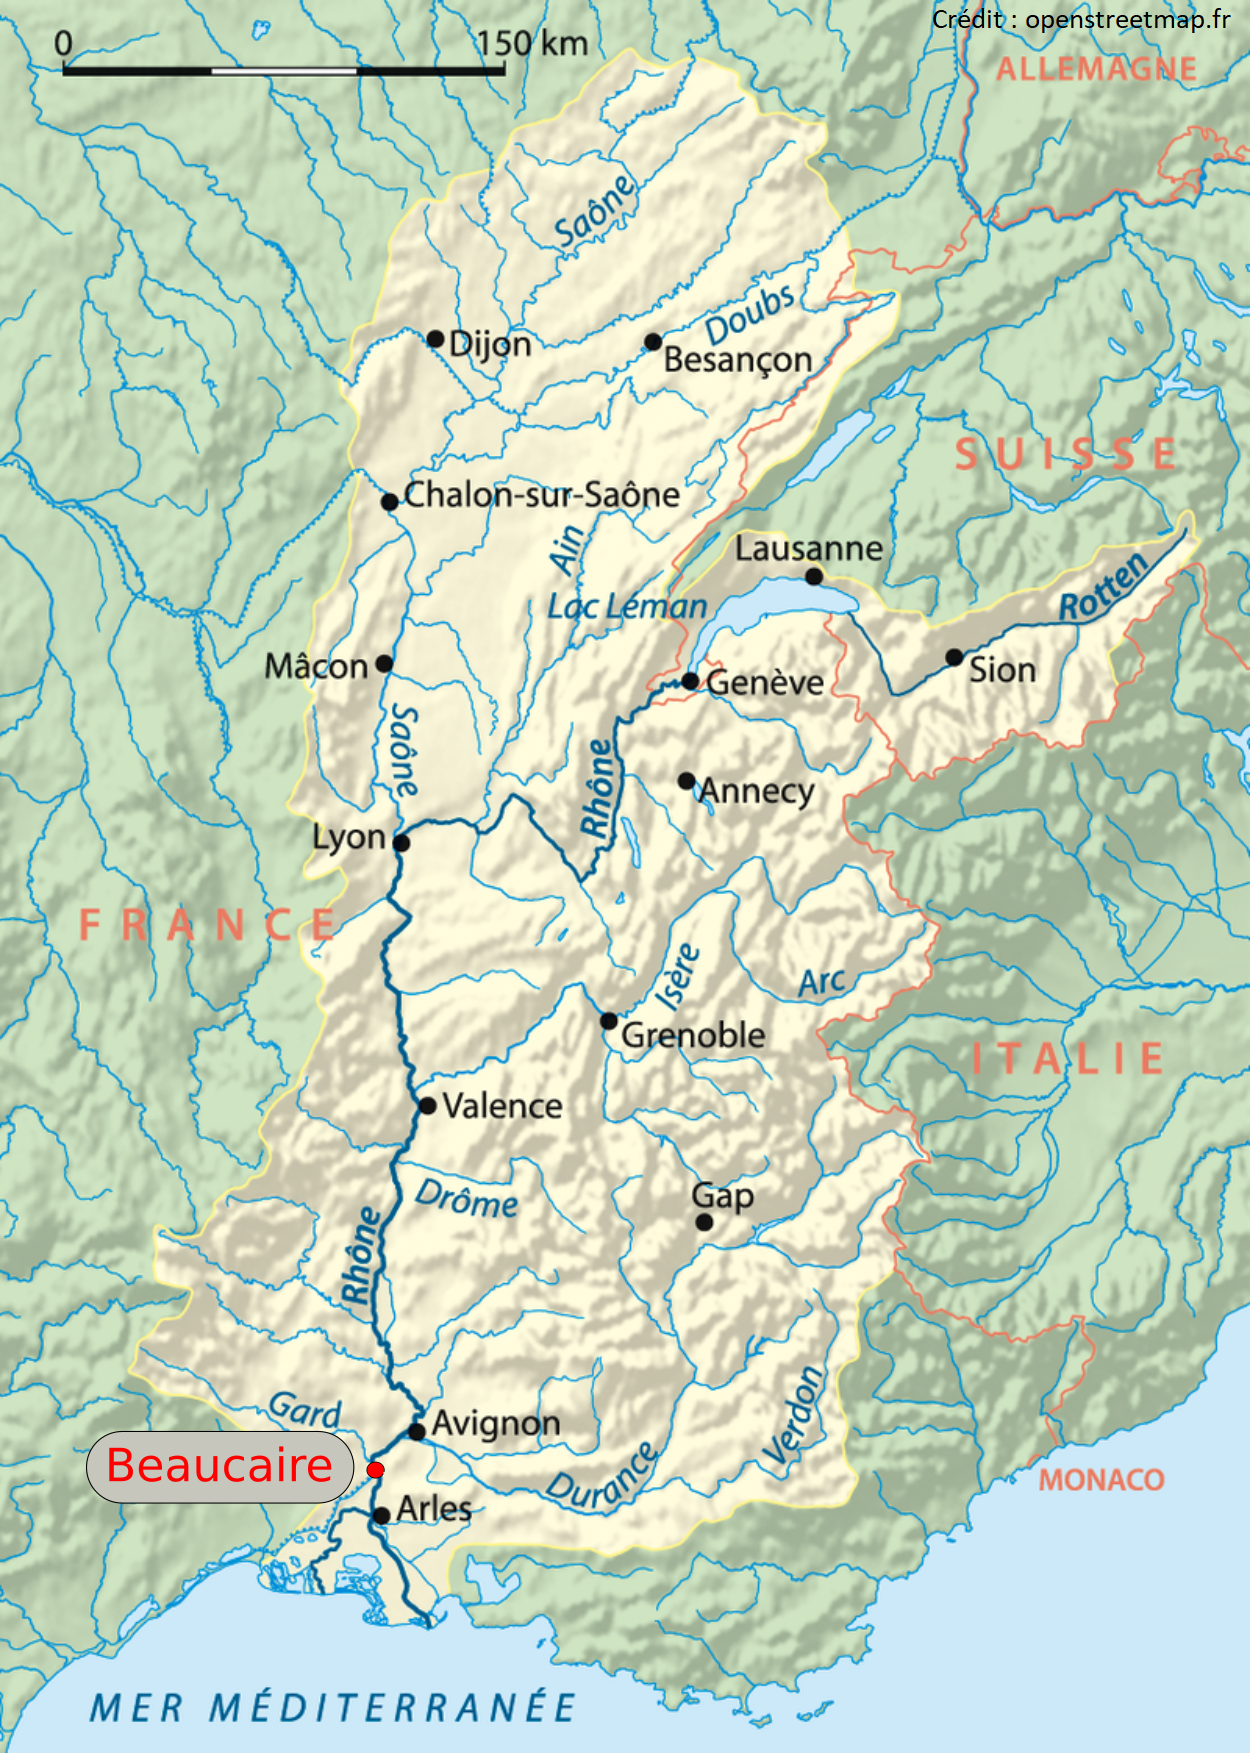
\includegraphics[width = \textwidth]{./Figures/Rhone_bassin_versant.png} 
		\end{minipage}
	\end{frame}
	
%	%%%%%%%%% 20 %%%%%%%%%
%	\begin{frame}%[c]
%		\frametitle{Régime hydrologique}
%		\centering
%      	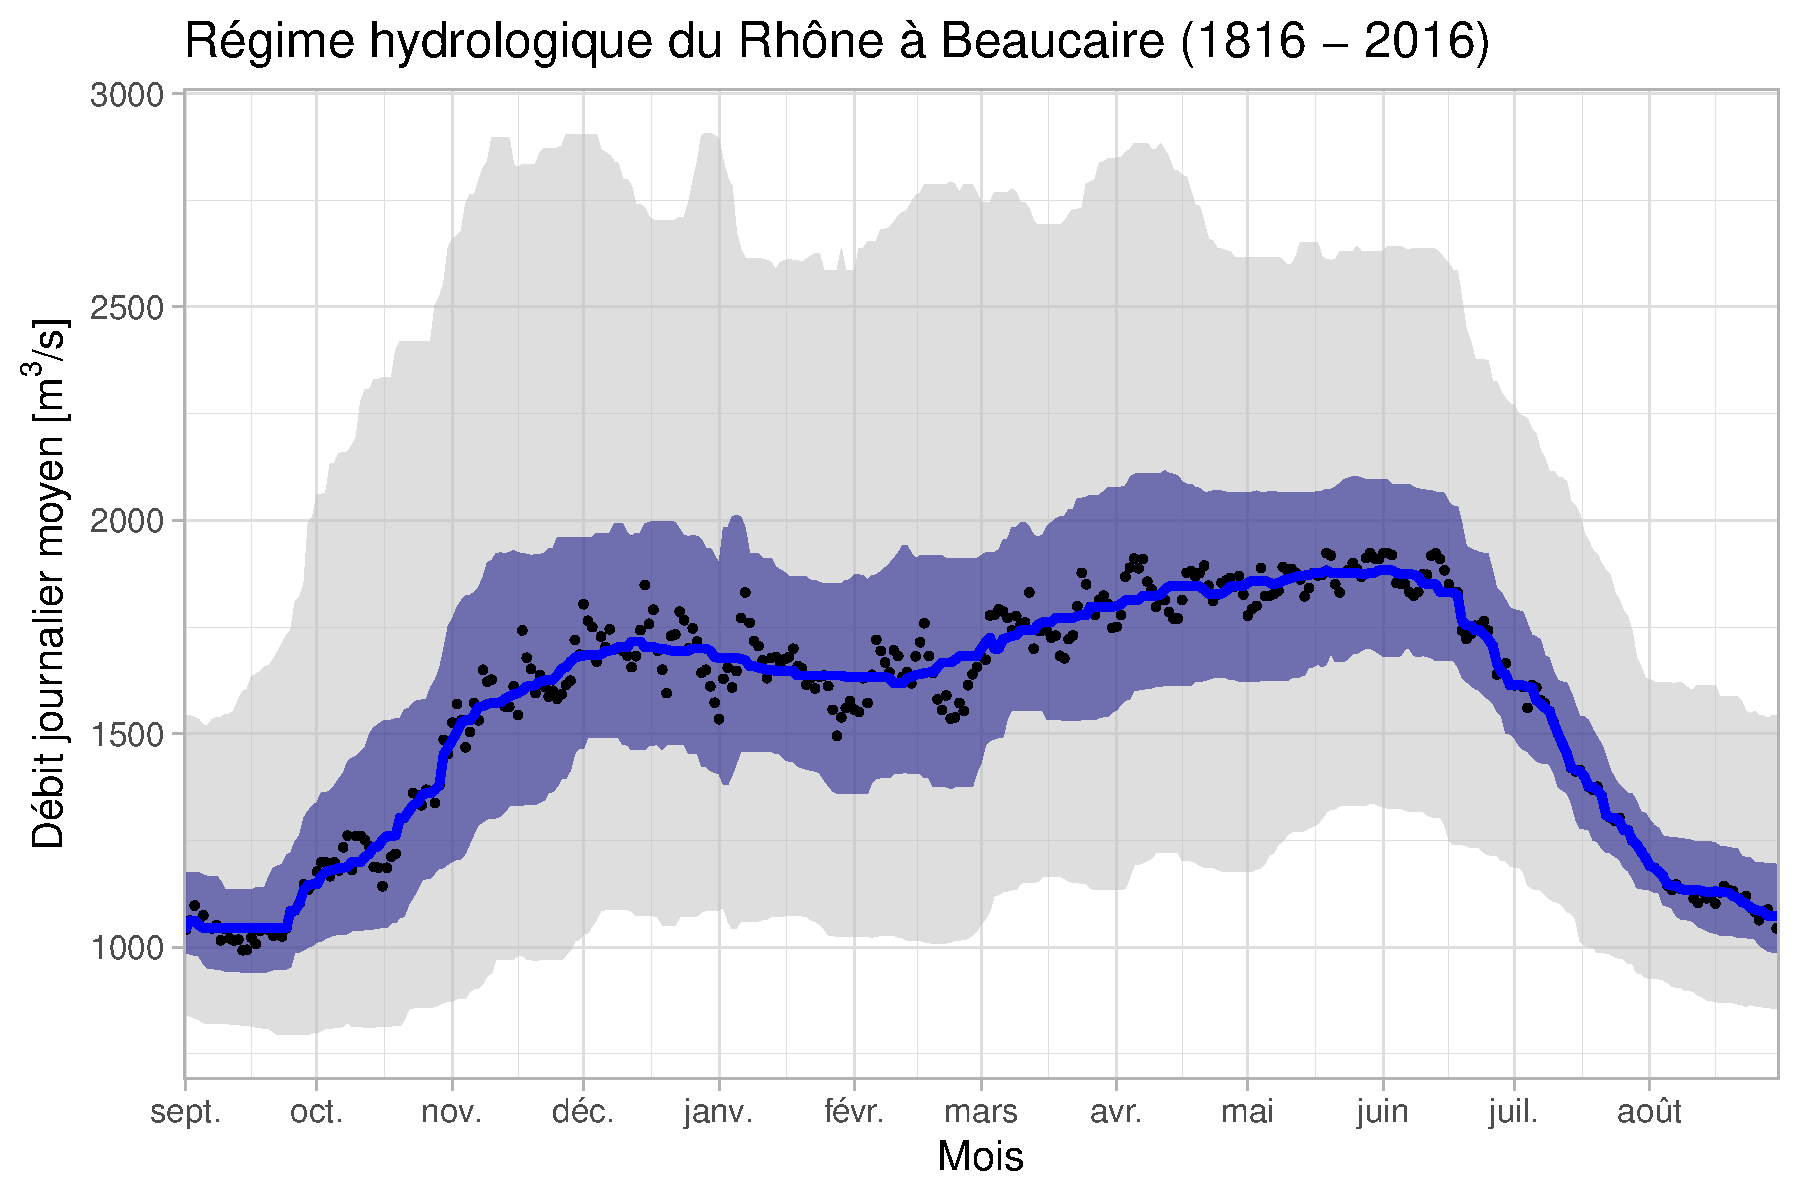
\includegraphics[width = .7\textwidth]{./Figures/Regime.pdf}\phantom{s}\\
%      	\centering     	
%      	Débits moyens journaliers et quantiles (20, 40, 60 et 80\%)
%	\end{frame}
%	
	%%%%%%%%% 21 %%%%%%%%%
	\begin{frame}%[c]
		\frametitle{Beaucaire et le Rhône}
		\begin{minipage}{.49\textwidth}
			\begin{itemize}
				\item<1->[$\vartriangleright$] Foire de Beaucaire : \og \textit{Capitale française des marchandises} \fg{}\footfullcite{leon_vie_1953}
				\vspace{5pt}
				\item<2->[$\vartriangleright$] Fortes crues au XIX\textsuperscript{ème} siècle
				\vspace{5pt}
				\item<3->[$\vartriangleright$] Début des relevés en 1816
				\vspace{5pt}
			\end{itemize}
		\end{minipage}
		\begin{minipage}{.49\textwidth}
			\begin{center}
	      		\includegraphics<1>[width = \textwidth]{./Figures/foire5.jpg} 
	      		\includegraphics<2>[width = \columnwidth]{./Figures/Napo.jpg} 
%	      		\includegraphics<3>[width = \columnwidth]{./Figures/Avi2003.jpg} 
	      		\includegraphics<3>[width = .6\textwidth]{./Figures/StationBcr.jpg} 
			\end{center}
		\end{minipage}
	\end{frame}
	
	%%%%%%%%% 22 %%%%%%%%%
	\begin{frame}%[c]
		\frametitle{Station hydrométrique (1816-2020)}
		\begin{minipage}{.45\textwidth}
			\begin{itemize}
				\item<1->[$\vartriangleright$] Relevés quotidiens dès 1816 : "\textbf{Pont de Beaucaire}"
				\vspace{2pt}
				\item<2->[$\vartriangleright$] Travaux CNR 1967-1970
				\vspace{2pt}
				\item<3->[$\vartriangleright$] Déplacement 2 km à l'aval : "\textbf{Beaucaire Restitution}"
				\vspace{2pt}
				\item<5->[$\vartriangleright$] Jaugeages dès 1845
			\end{itemize}
		\end{minipage}
		\begin{minipage}{.53\textwidth}
			\begin{center}
%	      		\includegraphics<1>[width = \textwidth]{./Figures/PtBcr.png} 
	      		\includegraphics<1>[width = \columnwidth]{./Figures/TabObs.jpg} 
%	      		\includegraphics<3-4>[width = \columnwidth]{./Figures/BcrRestit.png} 
	      		\includegraphics<5>[width = \textwidth]{./Figures/Jaus.pdf}
			\end{center}
		\end{minipage}
	\end{frame}
	
	\begin{frame}%[c]
		\frametitle{Station hydrométrique (1816-2020)}
		205 années de relevés systématiques de 1816 à 2020
		\vfill
		\includegraphics[width = .9\textwidth]{./Figures/carto.pdf} 
	\end{frame}
	
 	\subsection{HISTRHÔNE (1300-2000)}
	%%%%%%%%% 23 %%%%%%%%%
	\begin{frame}%[c]
		\frametitle{Base de données HISTRHÔNE (1300-2000)}
\begin{minipage}{.45\textwidth}
			\begin{itemize}
				\item<1->[$\vartriangleright$] Base de données d'événements hydroclimatiques en basse vallée du Rhône \footfullcite{pichard_sept_2014}
				\vspace{2pt}
				\item<2->[$\vartriangleright$] 1500 événements du XIII\textsuperscript{ème} siècle à 2000
				\vspace{2pt}
				\item<3->[$\vartriangleright$] Classés par type et par gravité 
			\end{itemize}
		\end{minipage}
		\begin{minipage}{.54\textwidth}
			\begin{center}
	      		\includegraphics<1-2>[width = .65\textwidth]{./Figures/HistrhoneMap.jpg} 
	      		\includegraphics<3>[width = .62\columnwidth]{./Figures/CatHistrhone.png}\phantom{s}\\
				\vspace{1pt}				
				\tiny{Tiré de \url{histrhone.cerege.fr}} 
			\end{center}
		\end{minipage}
	\end{frame}



{
    \setbeamercolor{background canvas}{bg=myblue}
    \begin{frame}
        \begin{center}
		 	\textcolor{white}{\large \textbf{Estimation des débits et incertitudes}}\\
		 	\vspace{0.8cm}
		 	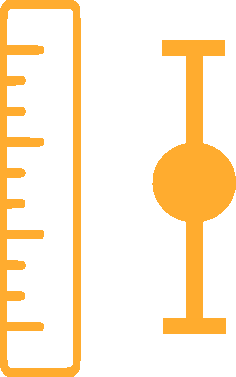
\includegraphics[width = .2\textwidth]{./Figures/LogoHydro.pdf} 
        \end{center}
    \end{frame}
    }
    
\section{Estimation des débits} 
	\subsection{Intro}
    \begin{frame}
    		\frametitle{Chaine de propagation des incertitudes}
    		\begin{center}
    			\includegraphics<1>[width = .7\textwidth]{./Figures/Serie2.pdf} 
      		\includegraphics<2>[width = .44\textwidth]{./Figures/SchemaProp1.pdf} 
			\includegraphics<3>[width = .44\textwidth]{./Figures/SchemaProp2.pdf} 
			\includegraphics<4>[width = .44\textwidth]{./Figures/SchemaProp3.pdf} 
%			\includegraphics<4>[width = .44\textwidth]{./Figures/SchemaProp0.pdf} 	
	     \end{center}
    \end{frame}
    
    \subsection{Courbes de tarage}
	\begin{frame}
		\frametitle{Détermination des \textit{a priori}}
		\begin{center}

		\end{center}	
	\end{frame}    
    
	\begin{frame}
		\frametitle{Segmentation des jaugeages}
		\begin{center}
%			\includegraphics<1>[width = .44\textwidth]{./Figures/SchemaProp1.pdf} 
			\includegraphics<1>[width = .7\textwidth]{./Figures/Jaus.pdf} 
			\includegraphics<2>[width = .7\textwidth]{./Figures/SegmPt.pdf} 
		\end{center}	
	\end{frame}
	
	\begin{frame}
		\frametitle{Estimation multipériode des courbes de tarage}
		\centering
		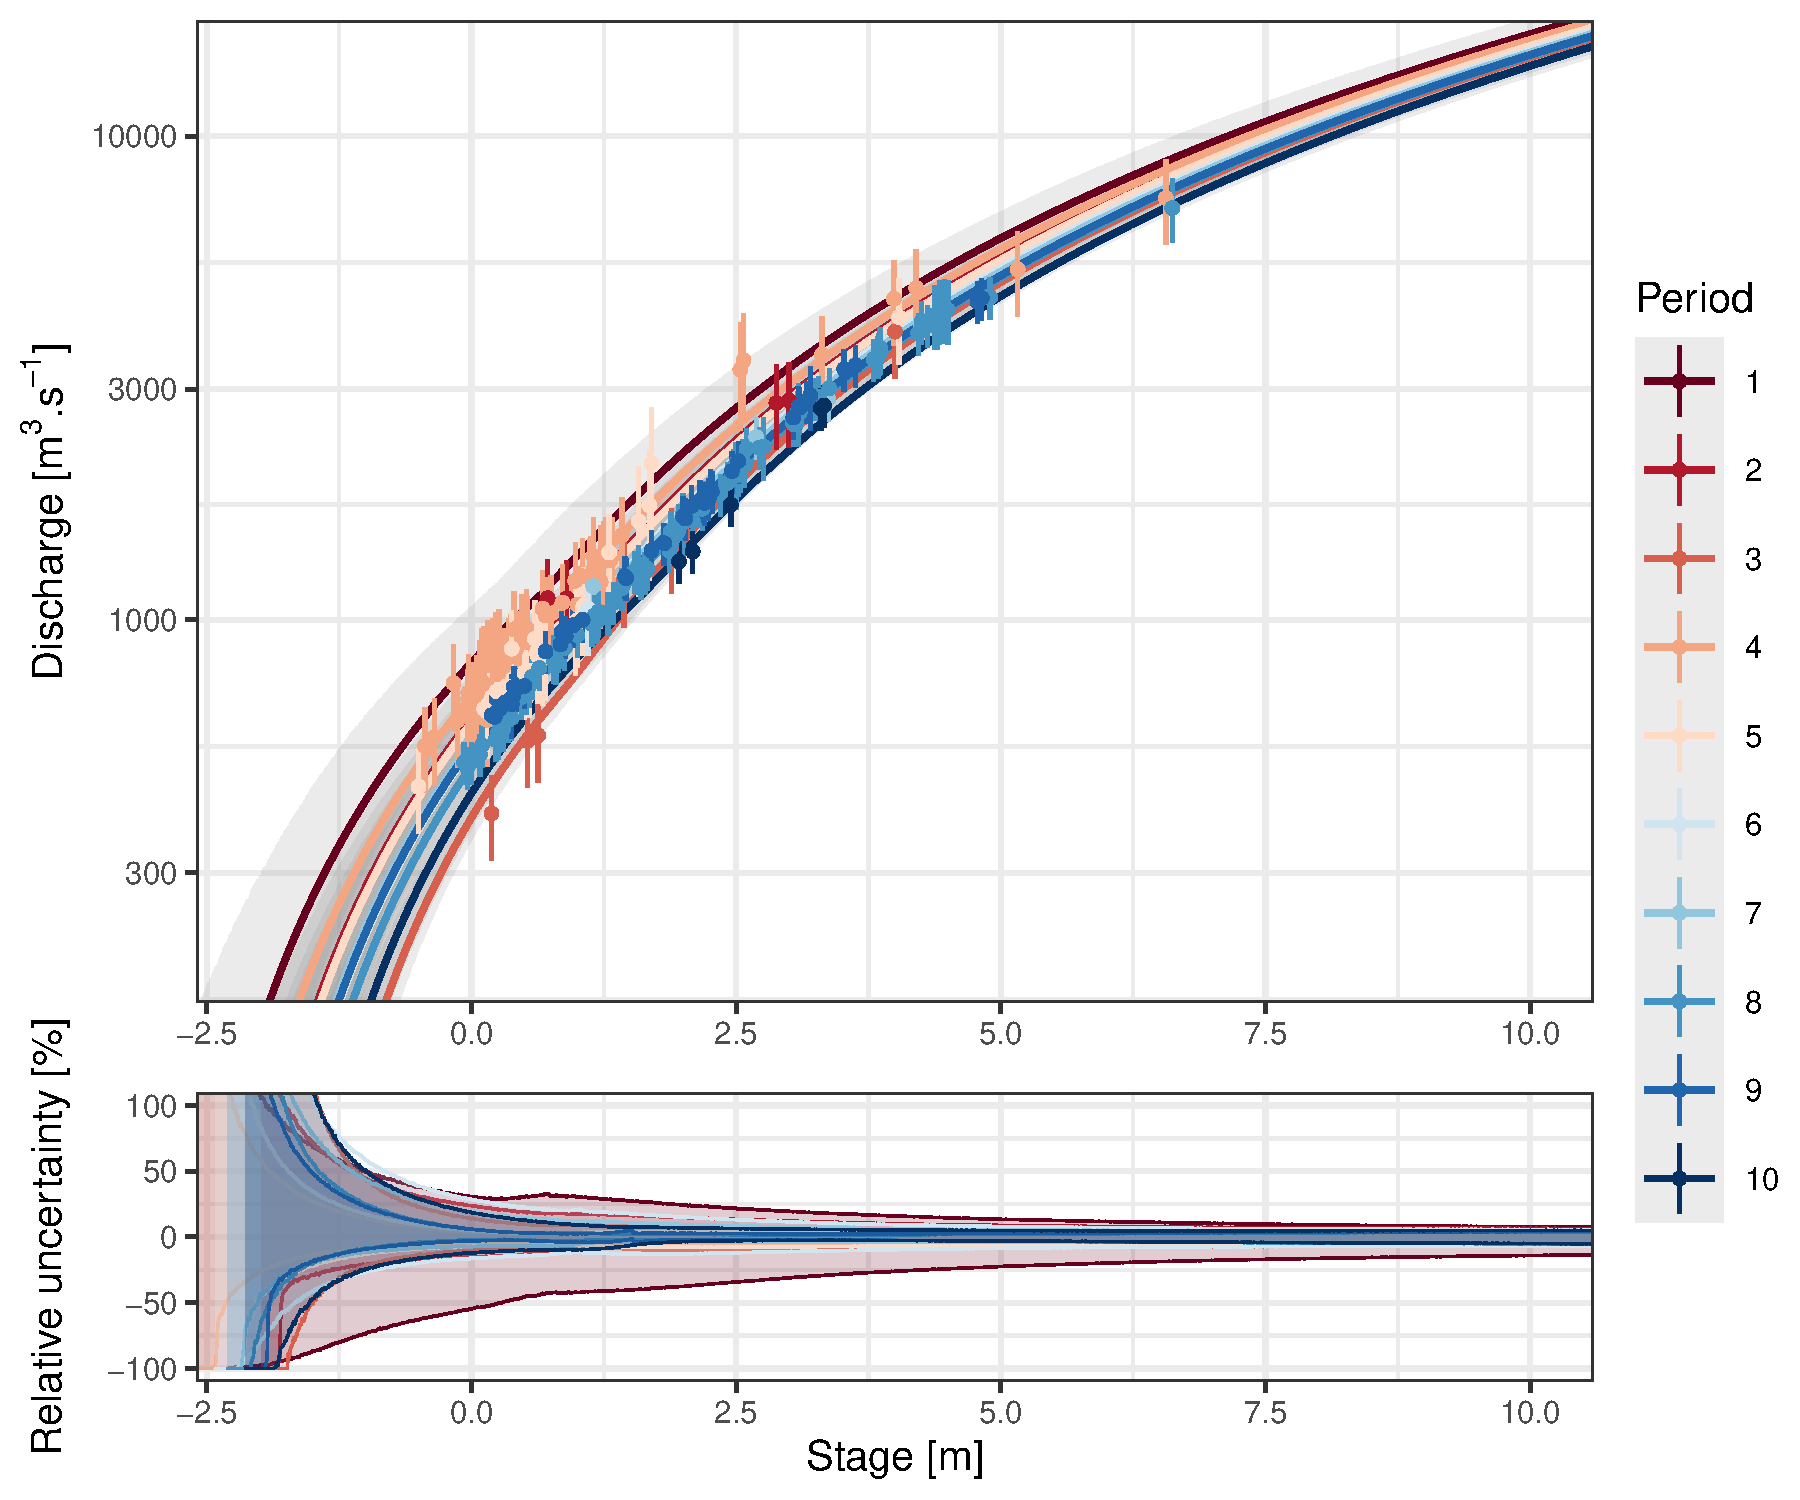
\includegraphics[width = .7\textwidth]{./Figures/RClog_ICdownPt.pdf}  	
	\end{frame}
	
	\subsection{Limnigrammes incertains}
	\begin{frame}
		\frametitle{Incertitude limnimétrique}
		\centering
		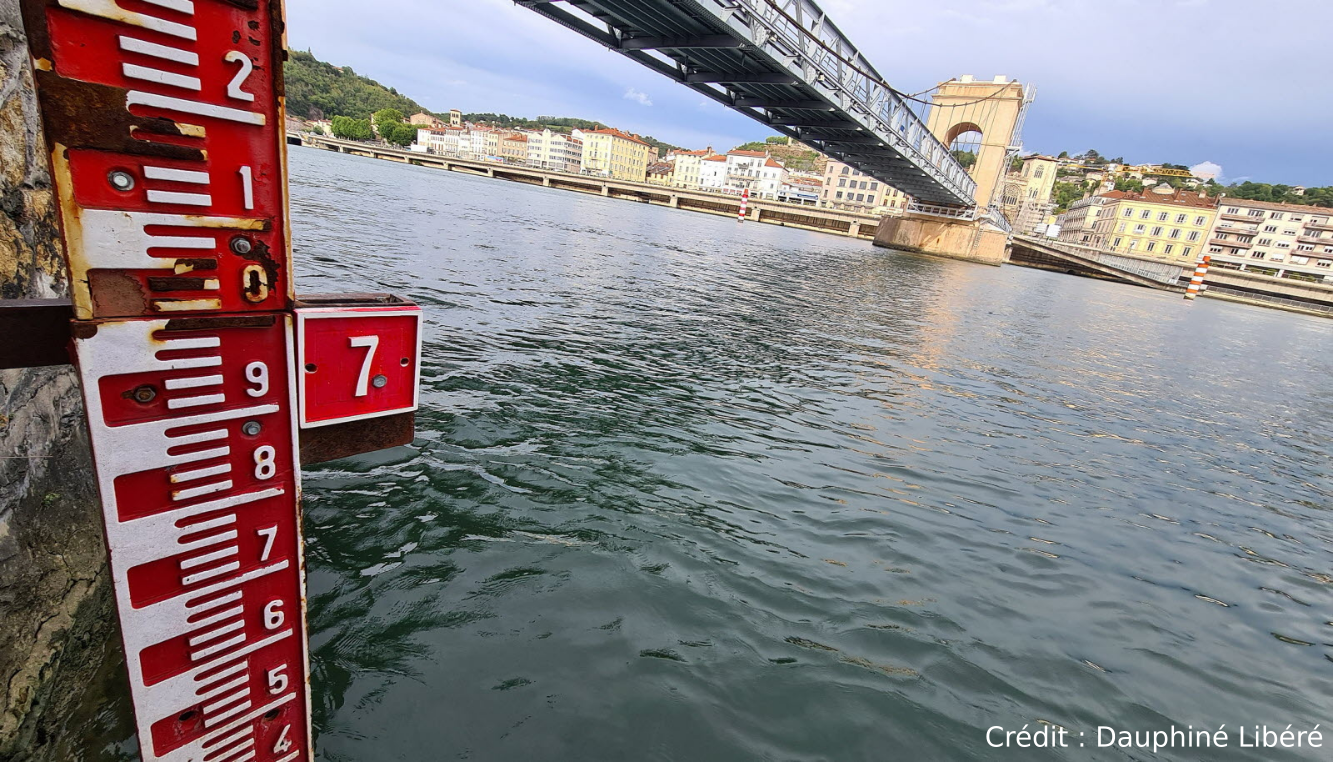
\includegraphics[width = .6\textwidth]{./Figures/LimniVienne.png}  	
	\end{frame}		
	
	\begin{frame}
		\frametitle{Incertitude limnimétrique}
		Incertitude composée de 5 erreurs additives : 
		\vspace{15pt}
		\begin{itemize}
			\item<2->[$\vartriangleright$] Lecture de l'échelle
			\item<3->[$\vartriangleright$] Appareil de mesure
			\item<4->[$\vartriangleright$] Calibration
			\item<5->[$\vartriangleright$] Mesure du zéro de l'échelle
			\item<6> [$\vartriangleright$] Fréquence des relevés 
		\end{itemize}
	\end{frame}	
	
	\begin{frame}
		\frametitle{Fréquence des relevés et interpolation}
		Avant 1840 : 1 mesure par jour à midi
		\vspace{15pt}
		\begin{itemize}
			\item<1> [$\vartriangleright$] Fréquence des relevés 
		\end{itemize}
	\end{frame}				
	
	\begin{frame}
		\frametitle{Incertitude limnimétrique}
		\centering
		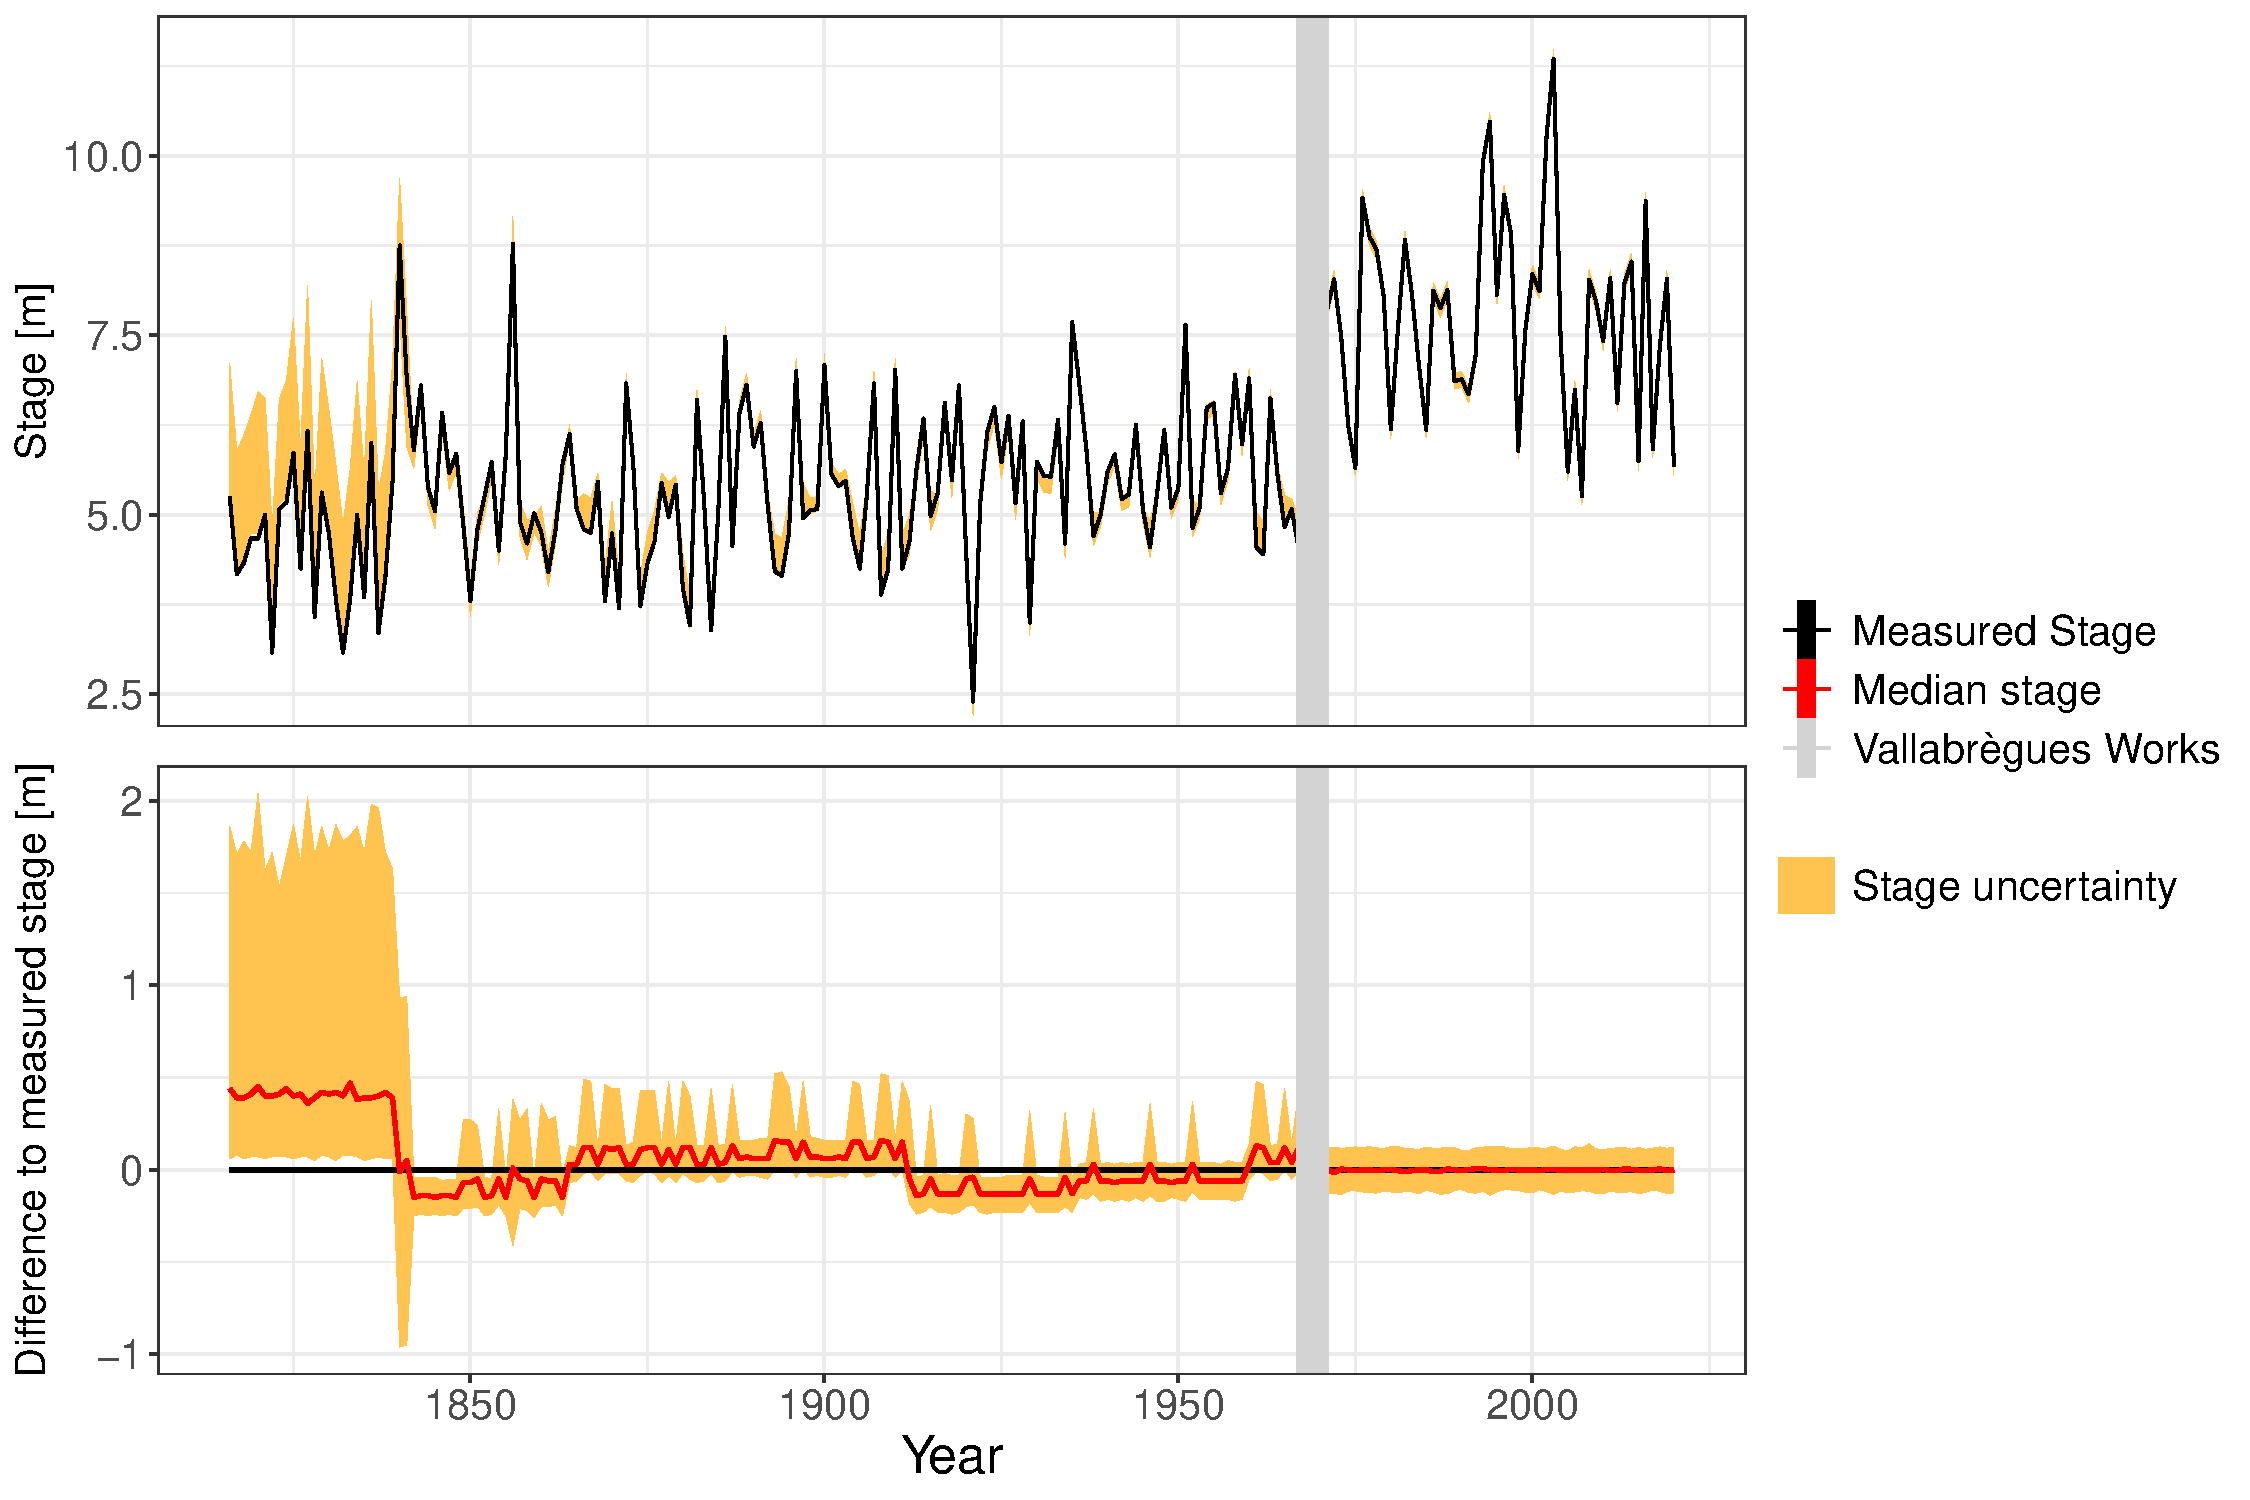
\includegraphics[width = .8\textwidth]{./Figures/8-StageErrorAMAX_BOTH.pdf} 
	\end{frame}	
	
	\begin{frame}
		\frametitle{Propagation des incertitudes}
		\centering
		\vspace{15pt}
		Propagation successive de chacune des sources d'incertitude 
		\vspace{10pt}
		\includegraphics<1>[width = .44\textwidth]{./Figures/SchemaProp3.pdf} 
		\includegraphics<2>[width = .85\textwidth]{./Figures/9-IcAndAMAX.pdf} 
	\end{frame}	
		
	\subsection{Témoignages de crues (1500-2000)}
	\begin{frame}
		\frametitle{Témoignages de crues}
		\centering
		\includegraphics<1>[width = .7\textwidth]{./Figures/Serie3.pdf} 		
	\end{frame}		
	
	\begin{frame}
		\frametitle{Témoignages de crues}
		\vspace{5pt}
		\textbf{Catégorie C4, crue et inondation
extrêmes} $\Rightarrow$ \og \textit{Inondation extraordinaire avec dégâts exceptionnels (pertes humaines et animales, intérieurs des villes inondés, dégradations de digues en grand nombre) et extension de crue}\fg{}  
	\vspace{15pt}
		\begin{itemize}
			\item<2->[$\vartriangleright$]  Ordre de grandeur ? \citet{pichard_hydro-climatology_2017} $\Rightarrow$ 9000 $m^3/s$ 
			\item<3>[$\vartriangleright$] Croisement avec les enregistrements systématiques de 1816 à 2020
		\end{itemize}
		\centering
		\includegraphics<4>[width = .8\textwidth]{./Figures/C4_SystematicPeriod-FR.pdf} 	
	\end{frame}		

	\subsection{Conclusion estimation débits}
	\begin{frame}
		\frametitle{Conclusions}
		\vspace{5pt}
		Données disponibles pour l'analyse fréquentielle :
		\begin{itemize}
			\item<1->[$\vartriangleright$] Estimation des débits de la période systématique
			\item<2->[$\vartriangleright$] Mentions de crues historiques et ordre de grandeur
		\end{itemize}
		\vspace{5pt}
		\centering
		\includegraphics<2->[width = .7\textwidth]{./Figures/EchMixteC4Bcr.pdf} 
	\end{frame}

\section{Analyse fréquentielle}
	\subsection{Intro}
	{
    \setbeamercolor{background canvas}{bg=myblue}
    \begin{frame}
        \begin{center}
		 	\textcolor{white}{\large \textbf{Analyse fréquentielle des crues sur 5 siècles}}\\
		 	\vspace{0.8cm}
		 	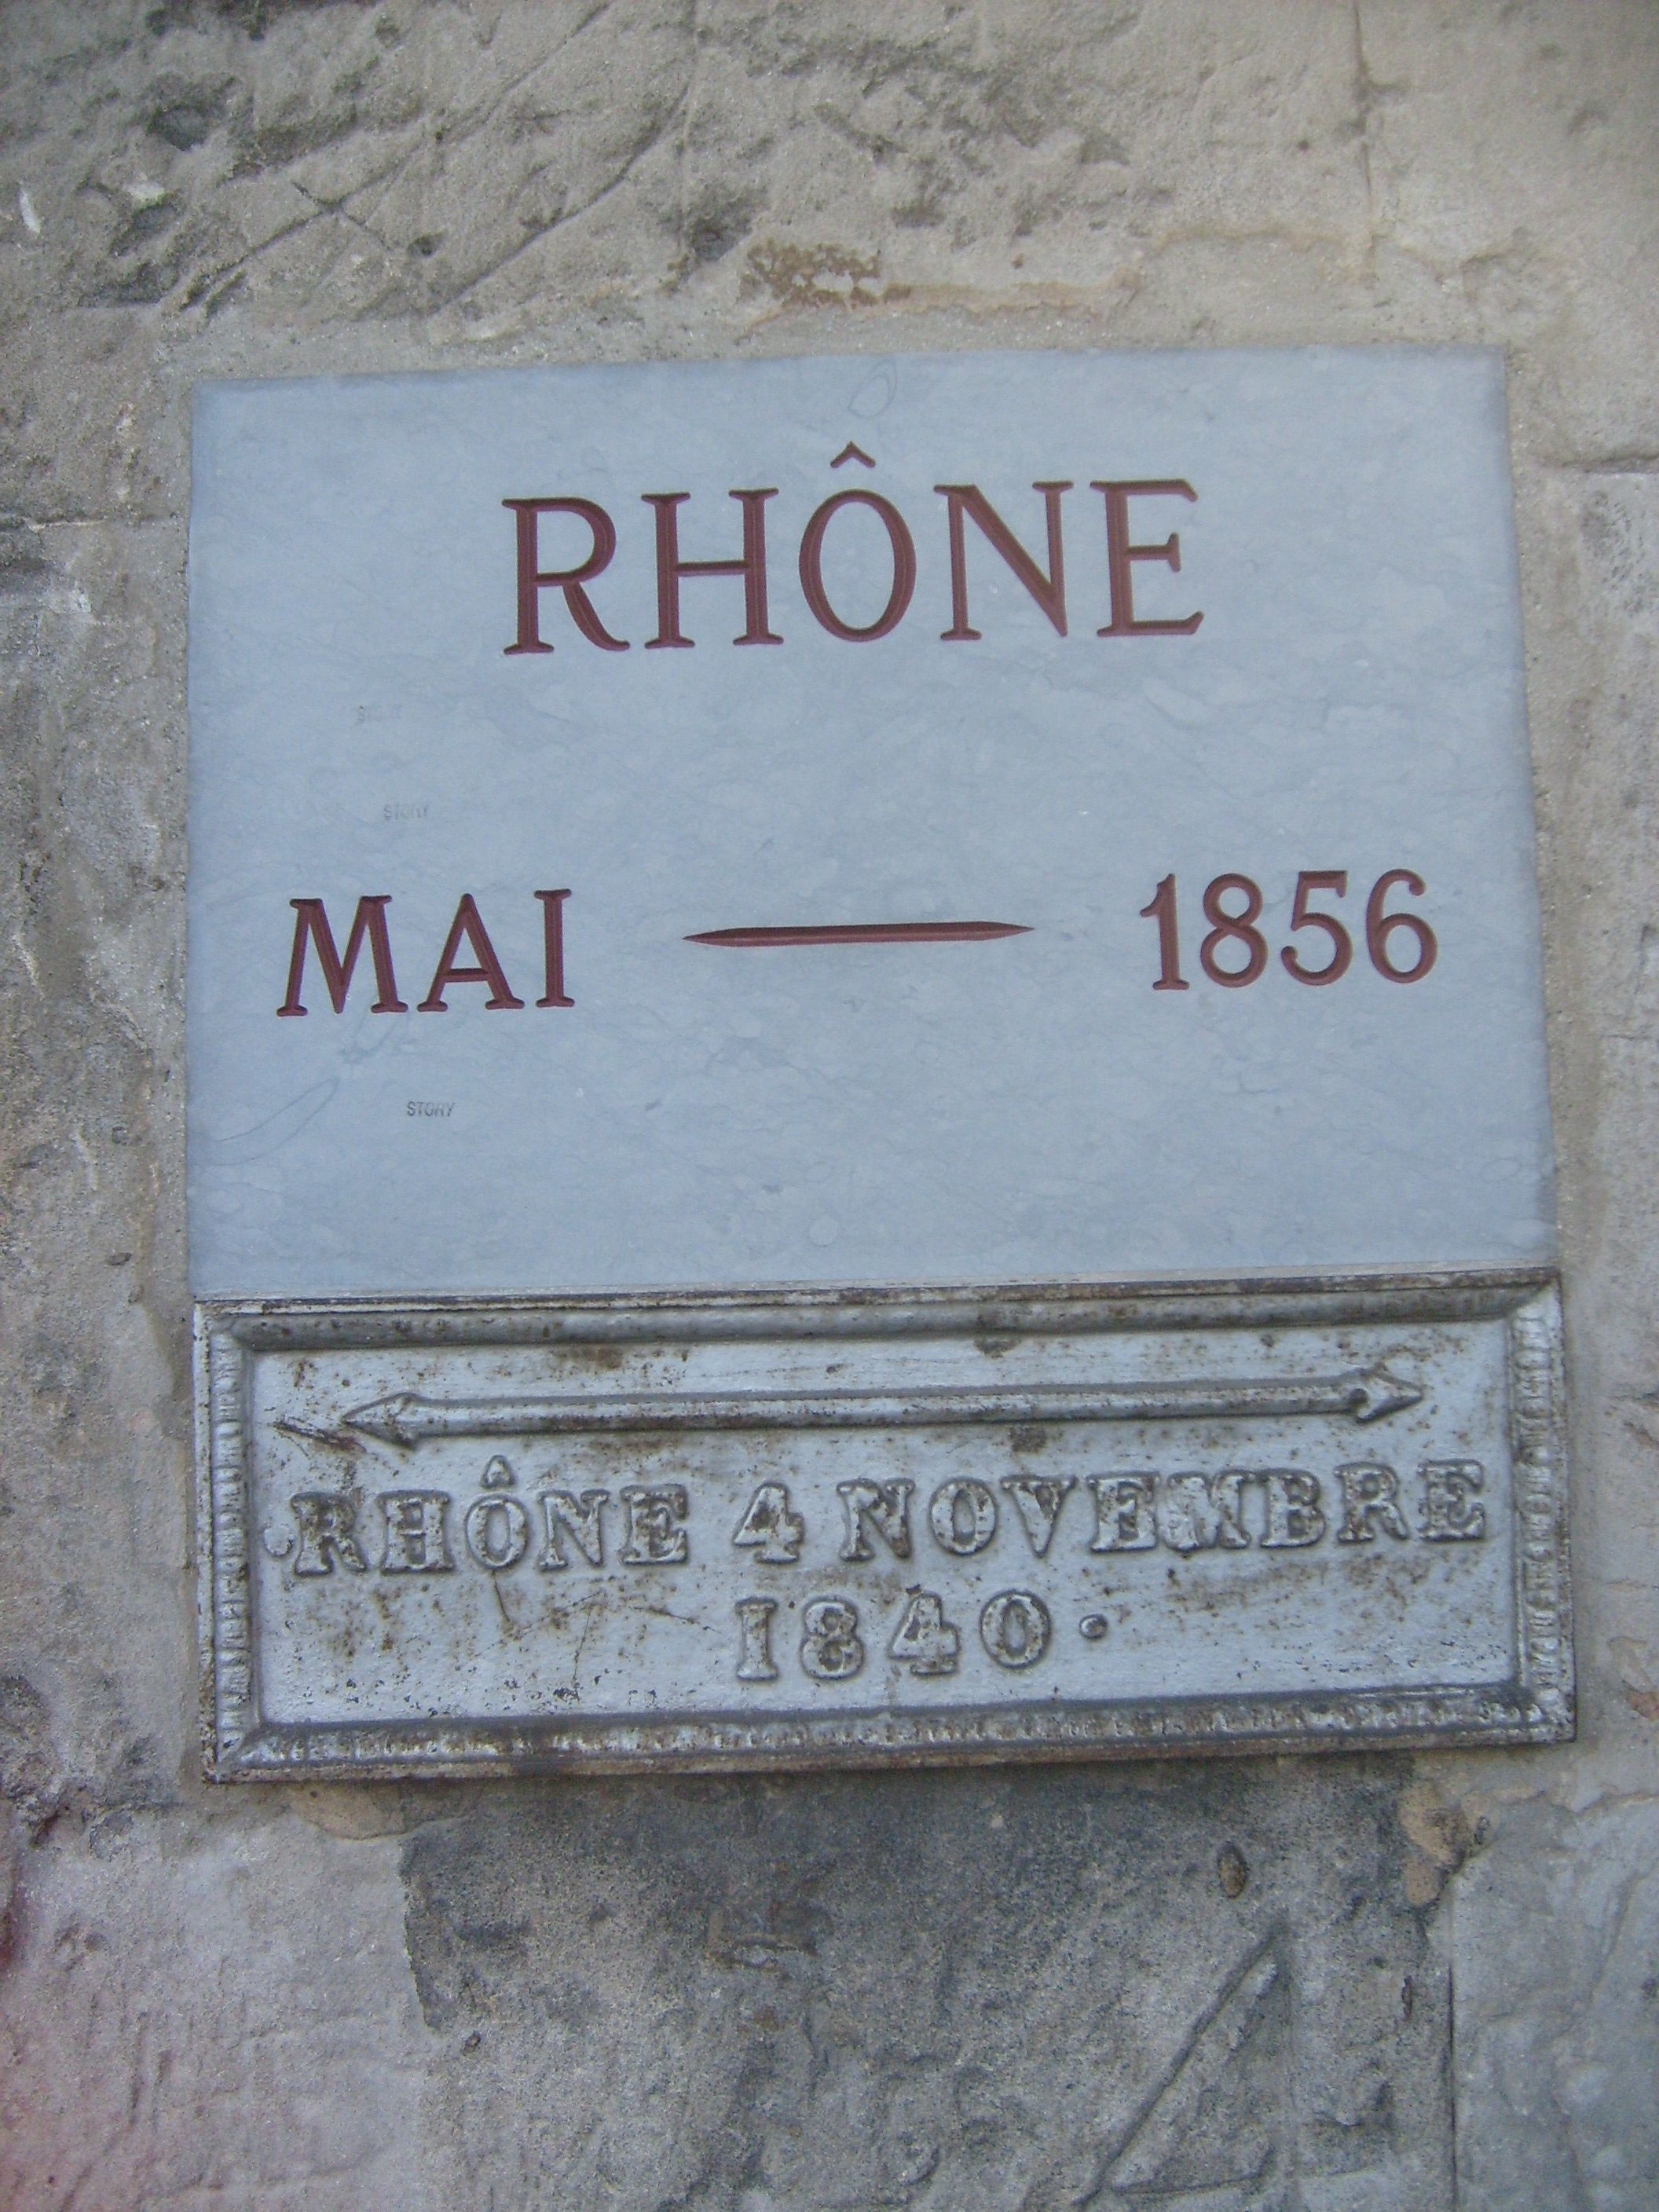
\includegraphics[width = .4\textwidth]{./Figures/RepAvi.jpg} 
        \end{center}
    \end{frame}
    }

	\subsection{Période systématique (1816-2020)}
	\begin{frame}
		\frametitle{Analyse fréquentielle 1816-2020}
		\centering
		\includegraphics<1>[width = .7\textwidth]{./Figures/EchMixteC4Bcr.pdf} 
	\end{frame}
	
	\begin{frame}
		\frametitle{Analyse fréquentielle 1816-2020}
		\vspace{5pt}
		2 types d'incertitude propagées indépendamment, puis successivement :\\
		\vspace{5pt}
		\begin{minipage}{.5\textwidth}
			\begin{itemize}
				\item<2->[$\vartriangleright$] Incertitude hydrométrique
					\vspace{40pt}
				\item<3->[$\vartriangleright$] Incertitude d'échantillonnage
			\end{itemize}
		\end{minipage}
		\begin{minipage}{.49\textwidth}
			\begin{center}
				\includegraphics<2->[width = .2\textwidth]{./Figures/LogoHydro.pdf} \phantom{s}\\
				\vspace{20pt}
				\includegraphics<3->[width = .3\textwidth]{./Figures/LogoSampling.pdf}		\phantom{s}\\	
			\end{center}	
		\end{minipage} 
		\vfill
		\centering
		\onslide<4> Quelle est la part de chacune des deux incertitudes dans l'incertitude totale des quantiles ? 
	 \end{frame}
	
	\begin{frame}
		\frametitle{Analyse fréquentielle 1816-2020}
		\centering
		\includegraphics<1>[width = \textwidth]{./Figures/10a-GeV_205years.pdf} 
		\includegraphics<2>[width = .9\textwidth]{./Figures/IC_AMAX_Both_Bands.pdf} 
		\includegraphics<3>[width = .8\textwidth]{./Figures/Ukplot4cases.pdf} 
		\includegraphics<4>[width = .8\textwidth]{./Figures/10e-Q1000SSize.pdf} 
	\end{frame}
	
	\subsection{Analyse d'un échantillon mixte}
	\begin{frame}
		\frametitle{Seuil de perception}
		\vfill
		Données de crues historiques $\Rightarrow$ données sporadiques : exhaustivité ?\\
		\vspace{5pt}
		Utilisation du concept de "seuil de perception" \footfullcite{gerard_probability_1979};\footfullcite{stedinger_flood_1986} :\\
		\vfill
		\begin{itemize}
			\item Crues > Seuil de perception $\Rightarrow$ apparaissent dans les données historiques
			\vfill
			\item Années sans mentions de crue < Seuil de perception
			\vfill
			\item Connaissance du débit des crues historiques $\Rightarrow$ pas nécessaire : nombre de dépassements du seuil suffisant \textsuperscript{16;}\footfullcite{payrastre_usefulness_2011}
		\end{itemize}
	\end{frame}

	\subsection{Analyse d'un échantillon mixte}
	\begin{frame}
		\frametitle{Méthodes d'analyse d'un échantillon mixte}
		\begin{itemize}
			\item $\boldsymbol{q}= (q_t)_{t=1,...,j}$ $\Rightarrow$ échantillon de débits maximum annuels sur $j$ années
			\vspace{5pt}
			\item $k$ dépassements du seuil de perception $S$ sur $n$ années
			\item Et donc : $n-k$ années sans dépassement du seuil $S$
		\end{itemize}
		\vfill
		Fonction de répartition GEV : 
		\begin{equation}
			F(x;\boldsymbol{\theta}) = e^{-(1-\xi(\frac{x - \mu}{\sigma}))^{1/\xi}}
		\end{equation}

		\vfill
		La probabilité du dépassement du seuil $S$ peut alors s'écrire :
		\begin{equation}
			\pi = \biggl( 1 - F(S;\boldsymbol{\theta})\biggl) = 1 - e^{-\biggl(1-\xi\bigl(\frac{S-\mu}{\sigma}\bigl)\biggl)^{1/\xi} }		
		\end{equation}
		\vfill
		On suppose que $k$ suit une loi binomiale de paramètres $n$ et $pi$ $\Rightarrow$ $\mathcal{B}(n,\pi)$
	
	\end{frame}		
		
	\begin{frame}
		\frametitle{Méthodes d'analyse d'un échantillon mixte}
		La vraisemblance de l'échantillon mixte s'écrit alors :
			\begin{equation}
			L(\boldsymbol{\theta} ; \boldsymbol{q}, k) = \underbrace{\prod_{t=1}^j f\left(q_t;\boldsymbol{\theta}\right)}_{\mathrm{période\,systématique}} \underbrace{\left\{\left(\begin{array}{l}
			n \\
			k
			\end{array}\right) F\left(S;\boldsymbol{\theta}\right)^{n-k}\left[1-F\left(S;\boldsymbol{\theta}\right)\right]^k\right\}}_{\mathrm{période\,historique}} 
			\end{equation}
			\vfill
			Formule de Bayes $\Rightarrow$ distribution des paramètres $\boldsymbol{\theta}$ sachant les données :
			\begin{equation}
				\underbrace{p(\boldsymbol{\theta} \mid \boldsymbol{q},k)}_{\mathrm{Paramètres GEV}} \propto \underbrace{L(\boldsymbol{\theta};\,\boldsymbol{q},k)}_{\mathrm{Vraisemblance}}  \underbrace{p(\boldsymbol{\theta})}_{{\mathrm{Données}} }
			\end{equation}
			\vfill			
			Distribution \textit{a posteriori} explorée via une méthode bayésienne MCMC \footfullcite{renard_application_2006}
	\end{frame}
	
	\subsection{Modèle fréquentiel historique}
	\begin{frame}
		\frametitle{Modèle A : propagation des incertitudes hydrométriques}
		Propagation des incertitudes hydrométriques de la période systématique
			\vfill
			$\boldsymbol{q}= (q_t)_{t=1,...,j}$ est remplacé par $(q_t^{(i)})_{t=1,...,j;\,i=1,...,s}$\\
			\vfill
			Un jeu de paramètres est ainsi estimé pour chacune des réalisations de $(q_t^{(i)})$\\
			\vfill
			Le résultat reflète incertitude hydrométrique et incertitude d'échantillonnage
	\end{frame}
	
	\begin{frame}
		\frametitle{Modèle B : incertitude autour du seuil de perception}
		Le seuil de perception est généralement considéré parfaitement connu $\Rightarrow$ optimiste ?\\
		\vfill
		Tests de sensibilité \footfullcite{stedinger_flood_1986}, \footfullcite{viglione_flood_2013}, \footfullcite{macdonald_reassessing_2014}, \footfullcite{payrastre_usefulness_2011}, \footfullcite{parkes_defining_2016} mais pas d'estimation de son incertitude
		\vfill
		Impact de la méconnaissance de $S$ sur les résultats : \\
		\begin{equation}
			L(\boldsymbol{\theta},\textcolor{red}{S} ; \boldsymbol{q}, k) = \underbrace{\prod_{t=1}^j f\left(q_t;\boldsymbol{\theta}\right)}_{\mathrm{période\,systématique}} \underbrace{\left\{\left(\begin{array}{l}
			n\\
			k
						\end{array}\right) F\left(S;\boldsymbol{\theta}\right)^{n-k}\left[1-F\left(S;\boldsymbol{\theta}\right)\right]^k\right\}}_{\mathrm{période\,historique}} 
		\end{equation}\\
		\vfill
		Cette méconnaissance est spécifiée dans la distribution \textit{a priori} de $S$
	\end{frame}
	
	\begin{frame}
		\frametitle{Modèle C : incertitude autour de la durée de la période historique}
		Durée de la période historique généralement considérée comme étant connue et parfois débutant à la date de la première
		\vfill
		Impact de la méconnaissance de $n$ sur les résultats : \\
		\vfill
		\begin{equation}
			L(\boldsymbol{\theta},\textcolor{red}{n} ; \boldsymbol{q}, k) = \underbrace{\prod_{t=1}^j f\left(q_t;\boldsymbol{\theta}\right)}_{\mathrm{période\,systématique}} \underbrace{\left\{\left(\begin{array}{l}
			n\\
			k
			\end{array}\right) F\left(S;\boldsymbol{\theta}\right)^{n-k}\left[1-F\left(S;\boldsymbol{\theta}\right)\right]^k\right\}}_{\mathrm{période\,historique}} 
		\end{equation}\\
		\vfill
		Cette méconnaissance est spécifiée dans la distribution \textit{a priori} de $n$
	\end{frame}
	
	\begin{frame}
		\frametitle{Modèle D : incertitude autour de $S$ et $n$}
		Impact de la méconnaissance de $S$ \textbf{et} $n$ sur les résultats : \\
		\vfill
		\begin{equation}
			L(\boldsymbol{\theta},\textcolor{red}{S},\textcolor{red}{n} ; \boldsymbol{q}, k) = \underbrace{\prod_{t=1}^j f\left(q_t;\boldsymbol{\theta}\right)}_{\mathrm{période\,systématique}} \underbrace{\left\{\left(\begin{array}{l}
			n\\
			k
			\end{array}\right) F\left(S;\boldsymbol{\theta}\right)^{n-k}\left[1-F\left(S;\boldsymbol{\theta}\right)\right]^k\right\}}_{\mathrm{période\,historique}} 
		\end{equation}\\
		\vfill
	\end{frame}
	
	\begin{frame}[c]
		\frametitle{Modèles proposés}
		\vfill
		4 modèles $\Rightarrow$ 4 hypothèses 
		\vfill
		\textit{A priori} peu informatifs :
		\begin{itemize}
			\item Seuil $S = 9000$ [m\textsuperscript{3}/s $\Rightarrow mathrm{N}(9000,2000)$ \\
			\vfill
			\item Date de début de la période historique $t^* = 1816 \Rightarrow \mathrm{U}(1340,1840)$ :\\
			Date de la première crue > $S$ - 500 ans
		\end{itemize}
		\vfill
		\begin{table}
			\centering
			\begin{tabular}{c|c|c|c|c}
	%			\hline
				Modèle & \textcolor{orange}{A} & \textcolor{red}{B} & \textcolor{cyan}{C} & \textcolor{blue}{D}\\\hline
				Seuil $S$ [m\textsuperscript{3}/s     & Connu 9000 & Incertain $\mathcal{{N}(9000,2000)$ & Connu 9000 & Incertain $\mathcal{N}(9000,2000)$ \\ \hline
				Date $t^*$ & Connue 1816 & Connue 1816 & Incertaine $\mathcal{U}(1340,1840)$ & Incertaine $\mathcal{U}(1340,1840)$ \\
			\end{tabular}
		\end{table}
	\end{frame}

	\subsection{Échantillon dégradé}
	
	\begin{frame}
		\frametitle{Test des modèles proposés}
		\vfill
		Test sur un échantillon artificiellement dégradé dont les paramètres sont connus\\
		\vspace{5pt}
		Soit $S = 9000$ $m^3/s$ et $n = 154$ ans\\
		\vfill
		\begin{itemize}
			\item Pont de Beaucaire (1816-1970) : Nombre de dépassements du seuil S = 9000 m\textsuperscript{3}/s
			\vspace{5pt}			
			\item Beaucaire Restitution (1971-2020) : L'ensemble des débits maximum annuels avec incertitude
		\end{itemize}
	\end{frame}
	
	\begin{frame}[c]
		\frametitle{Échantillon dégradé (1816-2020)}
		\begin{center}
			\includegraphics<1>[width = .5\textwidth]{./Figures/BarplotArtif0.pdf} 
			\includegraphics<2>[width = .5\textwidth]{./Figures/BarplotArtif1.pdf} 
			\includegraphics<3>[width = .5\textwidth]{./Figures/BarplotArtif2.pdf} 
			\includegraphics<4>[width = .5\textwidth]{./Figures/BarplotArtif3.pdf} 
			\includegraphics<5>[width = .5\textwidth]{./Figures/BarplotArtif4.pdf} 
			\includegraphics<6>[width = .5\textwidth]{./Figures/BarplotArtif5.pdf} 
			\includegraphics<7>[width = .5\textwidth]{./Figures/BarplotArtifFull.pdf} 
		\end{center}
	\end{frame}
	
	\begin{frame}[c]
		\frametitle{Échantillon dégradé (1816-2020)}
		\begin{center}
			\includegraphics<1>[width = .8\textwidth]{./Figures/Params_Artif2.pdf} 
			\includegraphics<2>[width = .6\textwidth]{./Figures/Shape_Artif2.pdf} 
		\end{center}
	\end{frame}
	
	\begin{frame}[c]
		\frametitle{Échantillon dégradé (1816-2020)}
		
		\begin{itemize}
			\item Méconnaissance de $S$ $\Rightarrow$ plus impactante que méconnaissance de $n$
			\vfill
			\item Distribution \textit{a posteriori} de $n$ relativement large
			\vfill
			\item Corrélations entre $S$ et $n$
		\end{itemize}
	\end{frame}
	
	\subsection{Échantillon complet}
	\begin{frame}[c]
		\frametitle{Échantillon complet (1500-2020)}
		\begin{center}
			\includegraphics<1>[width = .5\textwidth]{./Figures/BarplotC4Full.pdf} 
			\includegraphics<2>[width = .8\textwidth]{./Figures/Params_C4.pdf} 
			\includegraphics<3>[width = .6\textwidth]{./Figures/Shape_C4.pdf} 
		\end{center}
	\end{frame}
	
\subsection{Conclusion}
	\begin{frame}[c]
		\frametitle{Conclusion sur l'analyse fréquentielle de 1500 à 2020}
		\begin{center}
			bla
		\end{center}
	\end{frame}
	
\section{Conclusion générale}
	\subsection{Conclusion}
	\begin{frame}
		\frametitle{Conclusion}
		b
	\end{frame}

	\subsection{Perspectives}
	\begin{frame}
		\frametitle{Perspectives}
		b
	\end{frame}
	
%	\subsection{Remerciements}
%	hommage PICHARD

%\section{Bibliographie}
%	\begin{frame}
%		
%	\printbibliography
%
%	\end{frame}


%	\printbibliography

%\section{Annexes}	


\end{document}

